% По умолчанию используется шрифт 14 размера. Если нужен 12-й шрифт, уберите опцию [14pt]
\documentclass[14pt
  , russian
  %, xcolor={svgnames}
  ]{matmex-diploma-custom}
\usepackage[table]{xcolor}
\usepackage{graphicx}
\usepackage{tabularx}
\newcolumntype{Y}{>{\centering\arraybackslash}X}
\usepackage{amsmath}
\usepackage{amsthm}
\usepackage{amsfonts}
\usepackage{amssymb}
\usepackage{mathtools}
\usepackage{thmtools}
\usepackage{thm-restate}
\usepackage{tikz}
\usepackage{wrapfig}
% \usepackage[kpsewhich,newfloat]{minted}
% \usemintedstyle{vs}
\usepackage[inline]{enumitem}
\usepackage{subcaption}
\usepackage{caption}
\usepackage[nocompress]{cite}
\usepackage{makecell}
% \setitemize{noitemsep,topsep=0pt,parsep=0pt,partopsep=0pt}
% \setenumerate{noitemsep,topsep=0pt,parsep=0pt,partopsep=0pt}


\graphicspath{ {resources/} }

% 
% % \documentclass 
% %   [ a4paper        % (Predefined, but who knows...)
% %   , draft,         % Show bad things.
% %   , 12pt           % Font size.
% %   , pagesize,      % Writes the paper size at special areas in DVI or
% %                    % PDF file. Recommended for use.
% %   , parskip=half   % Paragraphs: noindent + gap.
% %   , numbers=enddot % Pointed numbers.
% %   , BCOR=5mm       % Binding size correction.
% %   , submission
% %   , copyright
% %   , creativecommons 
% %   ]{eptcs}
% % \providecommand{\event}{ML 2018}  % Name of the event you are submitting to
% % \usepackage{breakurl}             % Not needed if you use pdflatex only.
% 
% \usepackage{underscore}           % Only needed if you use pdflatex.
% 
% \usepackage{booktabs}
% \usepackage{amssymb}
% \usepackage{amsmath}
% \usepackage{mathrsfs}
% \usepackage{mathtools}
% \usepackage{multirow}
% \usepackage{indentfirst}
% \usepackage{verbatim}
% \usepackage{amsmath, amssymb}
% \usepackage{graphicx}
% \usepackage{xcolor}
% \usepackage{url}
% \usepackage{stmaryrd}
% \usepackage{xspace}
% \usepackage{comment}
% \usepackage{wrapfig}
% \usepackage[caption=false]{subfig}
% \usepackage{placeins}
% \usepackage{tabularx}
% \usepackage{ragged2e}
% \usepackage{soul}
\usepackage{csquotes}
% \usepackage{inconsolata}
% 
% \usepackage{polyglossia}   % Babel replacement for XeTeX
%   \setdefaultlanguage[spelling=modern]{russian}
%   \setotherlanguage{english}
% \usepackage{fontspec}    % Provides an automatic and unified interface 
%                          % for loading fonts.
% \usepackage{xunicode}    % Generate Unicode chars from accented glyphs.
% \usepackage{xltxtra}     % "Extras" for LaTeX users of XeTeX.
% \usepackage{xecyr}       % Help with Russian.
% 
% %% Fonts
% \defaultfontfeatures{Mapping=tex-text}
% \setmainfont{CMU Serif}
% \setsansfont{CMU Sans Serif}
% \setmonofont{CMU Typewriter Text}

\usepackage[final]{listings}

\lstdefinelanguage{ocaml}{
keywords={@type, function, fun, let, in, match, with, when, class, type,
nonrec, object, method, of, rec, repeat, until, while, not, do, done, as, val, inherit, and,
new, module, sig, deriving, datatype, struct, if, then, else, open, private, virtual, include, success, failure,
lazy, assert, true, false, end},
sensitive=true,
commentstyle=\small\itshape\ttfamily,
keywordstyle=\ttfamily\bfseries, %\underbar,
identifierstyle=\ttfamily,
basewidth={0.5em,0.5em},
columns=fixed,
fontadjust=true,
literate={->}{{$\to$}}3 {===}{{$\equiv$}}1 {=/=}{{$\not\equiv$}}1 {|>}{{$\triangleright$}}3 {\\/}{{$\vee$}}2 {/\\}{{$\wedge$}}2 {>=}{{$\ge$}}1 {<=}{{$\le$}} 1,
morecomment=[s]{(*}{*)}
}

\lstset{
mathescape=true,
%basicstyle=\small,
identifierstyle=\ttfamily,
keywordstyle=\bfseries,
commentstyle=\scriptsize\rmfamily,
basewidth={0.5em,0.5em},
fontadjust=true,
language=ocaml
}
 
\newcommand{\cd}[1]{\texttt{#1}}
\newcommand{\inbr}[1]{\left<#1\right>}


\newcolumntype{L}[1]{>{\raggedright\let\newline\\\arraybackslash\hspace{0pt}}m{#1}}
\newcolumntype{C}[1]{>{\centering\let\newline\\\arraybackslash\hspace{0pt}}m{#1}}
\newcolumntype{R}[1]{>{\raggedleft\let\newline\\\arraybackslash\hspace{0pt}}m{#1}}



\usepackage{soul}
\usepackage[normalem]{ulem}
%\sout{Hello World}

% перевод заголовков в листингах
\renewcommand\lstlistingname{Листинг}
\renewcommand\lstlistlistingname{Листинги}

\usepackage{afterpage}
\usepackage{pdflscape}
% TODO: Понять, почему я выделил то, что тут в отдельный файл
\usepackage{listings}
\usepackage{tikz}
\usetikzlibrary{decorations.pathreplacing,calc,shapes,positioning,tikzmark}

\newcounter{tmkcount}

\tikzset{
  use tikzmark/.style={
    remember picture,
    overlay,
    execute at end picture={
      \stepcounter{tmkcount}
    },
  },
  tikzmark suffix={-\thetmkcount}
}

\usepackage{caption}
\usepackage{listings}
\usepackage{graphicx}
\usepackage{multirow}
\usepackage{fancyvrb}
\usepackage[misc,geometry]{ifsym} 
\usepackage{subcaption}
\usepackage{multirow}
\usepackage{array}
\newcolumntype{P}[1]{>{\centering\arraybackslash}p{#1}}
\usepackage{tikz}
\usepackage{bbding}
\usepackage{pifont}
\usepackage{wasysym}
\usepackage{amssymb}
\usepackage{listings}
\usepackage{pythonhighlight}
\usepackage{tabularx}
\usepackage{array}
\usepackage{hyperref}
\newtheorem{definition}{Определение}

\DeclareCaptionFont{white}{ \color{white} }
\DeclareCaptionFormat{listing}{
    \parbox{\textwidth}{\hspace{15pt}#1#2#3}
}
\captionsetup[lstlisting]{ format=listing
  %, labelfont=white, textfont=white
  , singlelinecheck=false, margin=0pt, font={bf}
}

\setlength\extrarowheight{7pt}

\begin{document}
%% Если что-то забыли, при компиляции будут ошибки Undefined control sequence \my@title@<что забыли>@ru
%% Если англоязычная титульная страница не нужна, то ее можно просто удалить.
\filltitle{ru}{
    %% Актуально только для курсовых/практик. ВКР защищаются не на кафедре а в ГЭК по направлению, 
    %%   и к моменту защиты вы будете уже не в группе.
    chair              = {Кафедра системного программирования},
    group              = {19Б.10-мм},
    %
    %% Макрос filltitle ненавидит пустые строки, поэтому обязателен хотя бы символ комментария на строке
    %% Актуально всем.
    title              = {Разработка алгоритма для задачи достижимости с регулярными ограничениями},
    % 
    %% Здесь указывается тип работы. Возможные значения:
    %%   coursework - отчёт по курсовой работе;
    %%   practice - отчёт по учебной практике;
    %%   prediploma - отчёт по преддипломной практике;
    %%   master - ВКР магистра;
    %%   bachelor - ВКР бакалавра.
    type               = {practice},
    %
    %% Здесь указывается вид работы. От вида работы зависят критерии оценивания.
    %%   solution - <<Решение>>. Обучающемуся поручили найти способ решения проблемы в области разработки программного обеспечения или теоретической информатики с учётом набора ограничений.
    %%   experiment - <<Эксперимент>>. Обучающемуся поручили изучить возможности, достоинства и недостатки новой технологии, платформы, языка и т. д. на примере какой-то задачи.
    %%   production - <<Производственное задание>>. Автору поручили реализовать потенциально полезное программное обеспечение.
    %%   comparison - <<Сравнение>>. Обучающемуся поручили сравнить несколько существующих продуктов и/или подходов.
    %%   theoretical - <<Теоретическое исследование>>. Автору поручили доказать какое-то утверждение, исследовать свойства алгоритма и т.п., при этом не требуя написания кода.
    kind               = {solution},
    %
    author             = {Порсев Денис Витальевич},
    % 
    %% Актуально только для ВКР. Указывается код и название направления подготовки. Типичные примеры:
    %%   02.03.03 <<Математическое обеспечение и администрирование информационных систем>>
    %%   02.04.03 <<Математическое обеспечение и администрирование информационных систем>>
    %%   09.03.04 <<Программная инженерия>>
    %%   09.04.04 <<Программная инженерия>>
    %% Те, что с 03 в середине --- бакалавриат, с 04 --- магистратура.
    specialty          = {02.03.03 <<Математическое обеспечение и администрирование информационных систем>>},
    % 
    %% Актуально только для ВКР. Указывается шифр и название образовательной программы. Типичные примеры:
    %%   СВ.5006.2017 <<Математическое обеспечение и администрирование информационных систем>>
    %%   СВ.5162.2020 <<Технологии программирования>>
    %%   СВ.5080.2017 <<Программная инженерия>>
    %%   ВМ.5665.2019 <<Математическое обеспечение и администрирование информационных систем>>
    %%   ВМ.5666.2019 <<Программная инженерия>>
    %% Шифр и название программы можно посмотреть в учебном плане, по которому вы учитесь. 
    %% СВ.* --- бакалавриат, ВМ.* --- магистратура. В конце --- год поступления (не обязательно ваш, если вы были в академе/вылетали).
    programme          = {СВ.5006.2017 <<Математическое обеспечение и администрирование информационных систем>>},
    % 
    %% Актуально только для ВКР, только для матобеса и только 2017-2018 годов поступления. Указывается профиль подготовки, на котором вы учитесь.
    %% Названия профилей можно найти в учебном плане в списке дисциплин по выбору. На каком именно вы, вам должны были сказать после второго курса (можно уточнить в студотделе).
    %% Вот возможные вариканты:
    %%   Математические основы информатики
    %%   Информационные системы и базы данных
    %%   Параллельное программирование
    %%   Системное программирование
    %%   Технология программирования
    %%   Администрирование информационных систем
    %%   Реинжиниринг программного обеспечения
    % profile            = {Системное программирование},
    % 
    %% Актуально всем.
    %supervisorPosition = {проф. каф. СП, д.ф.-м.н., проф.}, % Терехов А.Н.
    supervisorPosition = {доцент кафедры информатики, к.ф.-м.н.,}, % Григорьев С.В.
    supervisor         = {Григорьев С.В.}
    % 

    % consultantPosition = {должность ООО <<Место работы>> степень},
    % consultant         = {К.К. Консультант}
}

\maketitle
\setcounter{tocdepth}{2}
\tableofcontents

% \begin{abstract}
%   В курсаче не нужен
% \end{abstract}

\section{Введение}
\paragraph{}
Графы являются одной из основных структур в информатике, а алгоритмы над ними чрезвычайно важны в анализе компьютерных и социальных сетей, статическом анализе кода, биоинформатике~\cite{gb_math}. Графы, возникающие в данных областях, могут содержать миллионы узлов и ребер, поэтому распараллеливание алгоритмов для работы с ними оказывается необходимым условием достижения высокой производительности. Однако такое улучшение их эффективности происходит за счет более сложной модели программирования~\cite{blast}. Результатом этого становится, в том числе, несоответствие между языками высокого уровня, на которых пользователи и разработчики графовых алгоритмов предпочли бы программировать (например, Python), и языками программирования для параллельного оборудования~\cite{blast}. Таким образом, существующие решения либо просты в использовании (networkx\footnote{Репозиторий библиотеки networkx: \url{https://github.com/networkx/networkx}. Дата посещения: 13.12.2020}), либо высокопроизводительны (gunrock\footnote{Репозиторий библиотеки gunrock: \url{https://github.com/gunrock/gunrock} Дата посещения: 13.12.2020}). Проблемой является и то, что традиционные параллельные алгоритмы для анализа графов тяжело реализовывать и оптимизировать, а прирост производительности от роста числа параллельных процессов снижается~\cite{gb_math}. 

С появлением эффективных структур и алгоритмов для разреженных матриц становится возможным использование подхода к вычислению над графами, основанного на линейной алгебре. Матрица смежности может представлять широкий спектр графов, включая ориентированные, взвешенные, двудольные. Ключевым свойством такого подхода является способность оперировать богатым набором графов различных типов с помощью небольшого набора матричных операций над полукольцами. Например, транспонирование матрицы смежности изменяет направления ребер в ориентированном графе, а умножение матрицы на вектор, как показано на рисунке~\ref{fig:bfs_step}, является шагом в алгоритме поиска в ширину.

\begin{figure}[h!]
    \centering
    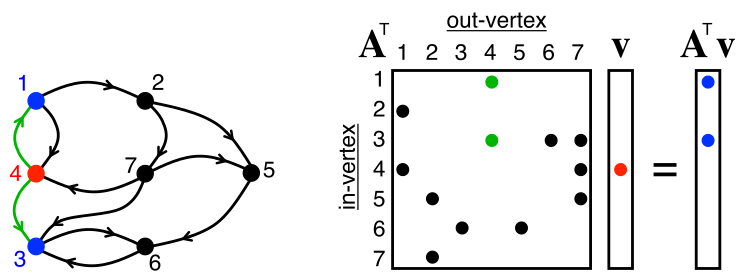
\includegraphics[width=0.9\linewidth]{pictures/MatrixBFS.png}
    \caption{Вычисление одного шага в алгоритме поиска в ширину\footnotemark}
    \label{fig:bfs_step}
\end{figure}

Спецификация GraphBLAS~\cite{gb_math} определяет базовые примитивы для построения графовых алгоритмов в терминах линейной алгебры. Разработчики считают, что эта область достаточно зрела, чтобы иметь потребность в стандартизации. Стандартизация позволяет сконцентрировать усилия исследователей на разработке инновационных алгоритмов для анализа и обработки графов, а не придумывать все новые, во многом пересекающиеся, низкоуровневые решения. Кроме того, благодаря такому подходу, по словам авторов\cite{sevengr}, возможно решение некоторых проблем, описанных ниже.
\begin{enumerate}
    \item \textbf{Переносимость.} Алгоритмы не требуют модификаций для достижения высокой производительности на конкретном устройстве.
    \item \textbf{Лаконичность.} Алгоритмы выражаются гораздо меньшим числом строчек кода.
    \item \textbf{Производительность.} Алгоритмы остаются высокопроизводительными.
    \item \textbf{Масштабируемость.} Алгоритмы эффективны как на небольших, так и на огромных данных.
\end{enumerate}

\footnotetext{GraphBLAS [Электронный ресурс] // Википедия. Свободная энциклопедия. – URL: \url{https://en.wikipedia.org/wiki/GraphBLAS} (дата обращения: 13.12.2020).}

GraphBLAS описывает небольшое множество математических операций, которые необходимы для реализации широкого спектра операций над графами. В стандарте описаны следующие объекты:
\begin{itemize}
    \item абстрактные структуры для хранения дынных (матрицы, векторы)
    \item алгебраические структуры (моноиды, полукольца, бинарные и унарные операторы)
    \item операции линейной алгебры над произвольными алгебраическими структурами (произведение матриц, поэлементное сложение и умножение, взятие подматрицы и т.д.)
    \item объекты управления (маски и дескрипторы)
\end{itemize}

На данный момент стандарт GraphBLAS уже имеет несколько полноценных реализаций\footnote{Форум, посвященный стандарту GraphBLAS: \url{https://graphblas.github.io/}. Дата посещения: 04.06.2021}, однако все они в основном ориентированы на исполнение на CPU. В то же время разработка инструмента с поддержкой исполнения на графических процессорах общего назначения является перспективным направлением исследований, так как их использование может существенно повысить производительность такого рода решений\cite{gbtl}\cite{blast}. На текущий момент нет стандартного подхода к реализации спецификации GraphBLAS на GPU --- разработчики сталкиваются не только с проблемами, связанными с реализацией обобщенных операций на графических процессорах с помощью стандартных инструментов языка C++, но и с переносимостью решений, основанных на программно-аппаратной платформе CUDA. Одним из возможных подходов к реализации GraphBLAS на GPU является использование языка высокого уровня, а также библиотек, динамически транслирующих конструкции и объекты данного языка в низкоуровневый код, способный исполнятся на графическом процессоре видеокарты. 


\section{Постановка задачи}
\label{sec:task}
Целью данной работы является исследование возможности применения подхода, основанного на комбинировании методов синтаксического анализа и машинного обучения, к задаче предсказания вторичной структуры молекулы РНК. Для реализации данной цели были поставлены следующие задачи.
\begin{itemize}
    \item Разработка архитектуры решения, конкретизирующей форматы анализируемых данных, а также используемые формальные грамматики и нейронные сети.
    \item Проведение экспериментальных исследований предложенной архитектуры, сравнение полученных результатов с существующими решениями.
\end{itemize}

\section{Обзор}
\label{sec:relatedworks}
Рассмотрим алгоритмы, решающие задачу поиска путей с контекстно-свободными ограничениями с помощью операций линейной алгебры, в несколько этапов. Первым этапом приведем определения, встречающиеся в их описании. Вторым этапом рассмотрим алгоритм, основанный на произведении Кронекера, и алгоритм, основанный на матричном умножении, и сравним их, выделяя проблемы, которые лягут в основу работы. Последним этапом выберем инструмент для оценки производительности решений указанных проблем.
\subsection{Базовые определения}

Следующее определение формально описывает структуру представления грамматики для алгоритма, основанного на произведении Кронекера.
\theoremstyle{definition}
\begin{definition}
Рекурсивный автомат \cite{rec} над конечным алфавитом $\Sigma$ есть набор $(M,m,\{C_i\}_{i \in M})$, где 

\begin{itemize}
    \item $M$ конечное множество меток,
    \item $m \in M$ начальная метка,
    \item $ \{C_i\}_{i \in M} $ множество \textit{конечных автоматов},
          где $C_i=(\Sigma \cup M, Q_i,q_i^0,F_i,\delta_i)$:
    \begin{itemize}
        \item $\Sigma \cup M$ множество символов, $\Sigma \cap M = \emptyset$,
        \item $Q_i$ конечное множество состояний,
              где $Q_i \cap Q_j = \emptyset, \forall i \neq j$,
        \item $q_i^0$ начальное состояние $C_i$,
        \item $F_i$ множество финальных состояний $C_i$, где $F_i \subseteq Q_i$,
        \item $\delta_i$ функция переходов $C_i$,
              где $\delta_i: Q_i \times (\Sigma \cup M)
              \to Q_i$.
    \end{itemize}
\end{itemize}
\end{definition}

\begin{definition}
Пусть $\mathcal{G}$ = $( \Sigma, $N$, $P$, $S$ )$ --- контекстно-свободная грамматика, тогда $\mathcal{G}$ находится в \textbf{ослабленной нормальной форме Хомского} (ОНФХ), если содержит только правила вида:
\begin{itemize}
    \item $A \rightarrow BC$, где $A$, $B$, $C \in N$
    \item $A \rightarrow a$, где $A \in N$, $a \in \Sigma$
    \item $A \rightarrow \varepsilon$, где $A \in N$
\end{itemize}
\end{definition}

Определение ОНФХ отличается от нормальной формы Хомского наличием правил вида $A \rightarrow \varepsilon$, где А --- любой нетерминал, то есть А не обязательно является стартовым, а также допущением использовать стартовый нетерминал в правых частях правил при наличии правила вида $S \to \varepsilon$.

\begin{definition}
Пусть $G$ --- помеченный граф с n вершинами, $M$ --- матрица смежности $G$ и $L$ --- множество различных меток на дугах графа $G$, тогда матрицей смежности для $l \in L$ называется матрица $M^l$ размером $n \times n$, где 
\begin{equation*}
M^l[i, j] = \begin{cases} true \text{, между вершинами i и j существует дуга с меткой } $l$\\ false \text{, иначе} \end{cases}    
\end{equation*} 
\end{definition}

\subsection{Алгоритм, основанный на произведении Кронекера}

В статье~\cite{10.1007/978-3-030-54832-2_6} был представлен алгоритм, основанный на произведении Кронекера, для поиска путей между всеми парами вершин, именуемый алгоритмом построения индекса, то есть результатом работы является структура данных, указывающая между какими парами есть требуемый путь. Представленный алгоритм основан на матричных операциях и использует рекурсивный автомат.

Алгоритм (листинг 2) принимает граф $G$ и рекурсивный автомат $R$. Основная идея заключается в использовании произведения Кронекера, как инструмента для пересечения двух автоматов. В качестве второго автомата в алгоритме предлагается выбрать граф $G$. Такой выбор является корректным, так как каждую вершину можно считать состоянием, а дуги --- переходами.

На начальном этапе (строки 2-3) алгоритма берутся матрицы смежности для всех меток графа и автомата по определению 1.3. Стоит отметить, что определение 1.3 дано для графа, но аналогичное определение можно ввести и для рекурсивного автомата. Дополнительно (строки 4-5) для каждого нетерминала из $R$ создается пустая матрица смежности в наборе $M_2$, который соответствует графу $G$.

Первым шагом (строки 6-9) проверяется наличие состояний в автомате $R$, которые одновременно являются стартовыми и конечными, то есть проверяется наличие $\varepsilon$ правил для грамматики. При наличии таковых из каждой вершины в неё же есть искомый путь.

Основной цикл (строки 10-20) алгоритма выполняется до тех пор пока набор матриц смежности для графа меняется. Первым шагом цикла происходит вычисление произведения Кронекера (строка 11), тем самым создавая матрицу смежности нового автомата. Далее результат транзитивно замыкается для получения информации о достижимости состояний в полученном автомате. И последним шагом (строки 14-20) происходит обновление при помощи операций, представленных на листинге 1, матрицы графа, которая соответствует нетерминалу, конечное состояние автомата которого достижимо из начального состояния.

%Алгоритм (листинг 2) принимает граф G и рекурсивный автомат R. Операции выполняются с булевской декомпозицией матриц смежности входных данных. Такой вид представления требует соответствующее переопределение операций, то есть операцией умножения будет являться логическое И, а операцией сложения --- логическое ИЛИ. Алгоритм состоит из трёх последовательных операций: произведение Кронекера, транзитивное замыкание и обновление. Произведение Кронекера пересекает два автомата (R и G), его результат транзитивно замыкается и на шаге обновления добавляются дуги с метками в виде соответствующих нетерминалов. Шаги алгоритма повторяются пока граф изменяется. На каждой итерации находятся пути длиной (количество дуг) на один больше чем на предыдущей.

%Алгоритм построения индекса, основанный на тензорном произведении, был представлен в статье~\cite{10.1007/978-3-030-54832-2_6}, который в рамках работы для краткости будет называться просто алгоритмом, основанным на Кронекеровом произведении. Он основан на матричных операциях, что позволяет использовать при его реализации высокопроизводительные библиотеки линейной алгебры. А также данный алгоритм использует рекурсивный автомат для представления грамматки, что дает ему преимущество по сравенению с алгоритмом~\cite{alg_matrix}, основанным на матричном умножении, так как второй принимает на вход грамматику лишь в ОНФХ, что приводит к её разрастанию, и, как следствие, отрицательно сказывается на производительности. Однако в процессе работы алгоритма, основанного на Кронекеровом произведении, а именно в результате Кронекерова произведения, возникают матрицы больших размеров. Например, если указанным образом перемножить одну матрицу размером $m \times p$ и вторую матрицу $n \times q$, то в результате получается матрица $mn \times pq$, что может отрицательно сказаться на производительности.

%Рассмотрим алгоритм подробнее. Пусть (см. листинг 2) $M_{1}$ --- набор матриц смежности меток для рекурсивного автомата, а $M_{2}$ --- набор матриц смежности для $\mathcal{G}$. При таком подходе каждой метке соответствует булева матрица смежности, то есть для какой-то метки A $M_{1}[A][i,j] = true$ означает наличие ребра из i в j с меткой A. Такой вид представления требует соответствующее переопределение операций, то есть операцией умножения будет являться логическое И, а операцией сложения --- логическое ИЛИ. Перед началом основного цикла алгоритма происходит постановка дуг среди вершин, среди которых существует путь длины 0. На первом же шаге основного цикла вычисляется Кронекерово произведение изначального автомата и графа, складывая все результаты Кронекерова произведения булевых матриц смежности из $M_{1}$ и $M_{2}$, соответствующих одним меткам. После чего результат транзитивно замыкается. Следующим шагом, обходя матрицу транзитивного замыкания, проверяется наличие ребра и принадлежность начальной и конечной вершин стартовому и конечному состоянию рекурсивного автомата, для этого на листинге 1 приведены вспомогательные функции. При выполнении условия алгоритм добавляет нетерминал/нетерминалы, соответствующие стартовому и конечному состоянию автомата, в ячейку матрицы из $M_{2}$, что свидетельствует о существовании пути, объединение меток которого выводится из указанного нетерминала, между индексами (вершинами) этой ячейки. Данные шаги алгоритма повторяются, пока одна из матриц в $M_{2}$ изменяется. Таким образом, за каждую итерацию $i$ получаются пути, выводимые из грамматики за $i$ шагов. Результатом работы алгоритма является набор матриц $M_{2}$.

\begin{algorithm}[H]
\floatname{algorithm}{Listing}
\begin{algorithmic}[1]
\caption{Вспомогательные функции}
\label{tensor:cfpq:help}
\Function{getStates}{$M_1, i, j$}
    \State{$r \gets dim(M_1)$}
    \State \Return{$\left\lfloor{i / r}\right\rfloor, \left\lfloor{j / r}\right\rfloor$}
\EndFunction
\Function{getCoordinates}{$M_2, i, j$}
    \State{$n \gets dim(M_2)$}
    \State \Return{$i \bmod n, j \bmod n$}
\EndFunction
\end{algorithmic}
\end{algorithm}

\begin{algorithm}[H]
\floatname{algorithm}{Listing}
\begin{algorithmic}[1]
\caption{Алгоритм, основанный на произведении Кронекера}
\label{tensor:cfpq}
\Function{contextFreePathQuerying}{$G$, $R$}
    % Input data preparation
    \State{$M_1 \gets$ набор матриц смежности для $R$}
    \State{$M_2 \gets$ набор матрица смежности для $G$}
    
    \ForAll{$nonterminals \in R$}
        \State{$M_2 = M_2 \cup \{\text{пустая матрица}\}$}
    \EndFor
    
    % Eps-transition handling for graph
    \For{$s \in 0..dim(\mathcal{M}_1)-1$}
        \For{$S \in \textit{getNonterminals}(R,s,s)$}
            \For{$i \in 0..dim(\mathcal{M}_2)-1$}
                \State{$M_2^S[i,i] \gets \{1\}$}
            \EndFor
        \EndFor
    \EndFor
    \While{Набор $M_2$ изменяется}
        \State{$M_3 \gets M_1 \otimes M_2$}
        \State{$C_3 \gets \textit{transitiveClosure}(M_3)$}
        \State{$n \gets$ dim($M_3)$}
        % Add non-terminals (possibly new)
        \For{$i \in 0..n-1$}
           \For{$j \in 0..n-1$}
                \If{$C_3[i,j]$}
                    \State{$s, f \gets \textit{getStates}(C_3,i,j)$}
                    \State{$x, y \gets \textit{getCoordinates}(C_3,i,j)$}
                    \For{$Nonterm \in \textit{getNonterminals}(R,s,f)$}
                        \State{$M_2^{Nonterm}[x,y] \gets \{1\}$}
                    \EndFor
                \EndIf
           \EndFor
        \EndFor
    \EndWhile
\State \Return $M_2$
\EndFunction
\end{algorithmic}
\end{algorithm}

Из рассмотренного видно, что на каждой итерации основного цикла происходит пересчет шагов, связанных с вычислениями произведения Кронекера и транзитивного замыкания. Хотя алгоритм обладает монотонностью, то есть добавленные дуги, свидетельствующие о существовании пути, никогда не удаляются из графа. То есть в пересчете заново указанных шагов нет никакой необходимости. Таким образом, появляется потребность в улучшении алгоритма построения индекса.

\subsection{Алгоритм, основанный на матричном умножении}

Вторым алгоритмом, основанным на операциях линейной алгебре, является алгоритм, основанный на матричном умножении, предложенный в статье~\cite{alg_matrix}. В качестве входных данных алгоритм принимает грамматику в ОНФХ и граф, который представлен также в виде набора булевых матриц смежности для каждой метки.

Основная идея алгоритма заключается в рассмотрении отдельно правил, где в правой части находится один терминал, вида $A \rightarrow a$, и правил, где в правой части находятся два нетерминала, вида $A \rightarrow BC$. Для первого типа правил о наличии искомого пути говорит наличие дуги с меткой в виде терминала $a$. Для второго типа правил предлагается умножать матрицы смежности, соответствующие двум нетерминалам $B$ и $C$. Такая операция позволяет соединить дугой вершины, которые достижимы путем, состоящим из 2 дуг, первая из которых с меткой $B$, а вторая --- с $C$, тем самым гарантируя обнаружение путей, выводимых из нетерминала $A$.

Было предложено множество модификаций этого алгоритма, покрывающие разнообразные варианты практического использования. Например, в статье Арсения Терехова и др.~\cite{ms-matrix} была предложена модификация, позволяющая искать пути, исходящих из фиксированного набора вершин.

\subsection{Сравнение алгоритмов, основанных на операциях линейной алгебры}

В предыдущих разделах были рассмотрены алгоритм, основанный на произведении Кронекера, и алгоритм, основанный на матричном умножении, реализации которых далее в работе будут обозначены Tns и Mtx, соответственно. Теперь рассмотрим их достоинства и недостатки перед друг другом.

Недостатком алгоритма, основанного на матричном умножении, является представление грамматики в виде ОНФХ, так как это влечёт к увеличению количества правил, что может отрицательно сказаться на производительности. В свою очередь алгоритм, основанный на произведении Кронекера, использует рекурсивный автомат, что является его преимуществом перед аналогом, так как позволяет избежать необходимости преобразовывать исходную грамматику. Однако алгоритм, основанный на произведении Кронекера, оперирует в процессе работы матрицами больших размеров, а именно в результате выполнения произведения Кронекера, взяв матрицу размера $m \times n$ в качестве второго операнда, получается матрица, количество строк и столбцов которой равно количеству строк и столбцов первого операнда увеличенных в $m$ и $n$ раз соответственно. 

Таким образом, оба алгоритма основаны на операциях линейной алгебре, что позволяет использовать высокопроизводительные библиотеки при их реализации. Однако алгоритм, основанный на произведении Кронекера, использует рекурсивный автомат, тем самым не увеличивает количество продукций исходной грамматики, что говорит о его конкурентоспособности перед алгоритмом, основанным на матричном умножении.

Но также важным достоинством алгоритма, основанного на матричном умножении, перед аналогом является наличие модификаций для извлечения путей и обнаружения путей, исходящих из фиксированного набора вершиин, так как их существование дает возможность полноценного использования алгоритма, например, в графовых базах данных. Таким образом, появляется потребность в разработке указанных модификаций для алгоритма, основанного на произведении Кронекера.

%Основная идея алгоритма заключается в интерпретации умножения матриц следующим образом. Рассмотрим умножение двух матриц: $C = A\times B$. Пусть эти две матрицы являются булевыми матрицами смежности. В таком случае, если переопределить операции умножения и сложения самих элементов матриц, а именно, операцию сложения заменить на логическое ИЛИ, а операцию умножения --- на логическое И, то полученная матрица $C$ будет булевой матрицей смежности графа, имеющего ребро $(i,j)$, если вершина i в A и вершина j в B имеют общую соседнюю вершину. Используя эту идею алгоритм, основанный на матричном умножении, обнаруживает искомые пути.



\subsection{Библиотека SuiteSparse}

Для реализации полученных алгоритмов и последующей оценки их производительности был выбран API GraphBLAS\footnote{Репозиторий проекта GraphBLAS: https://github.com/GraphBLAS Дата посещения: 25.12.2020}, так как на данный момент является единственным API для работы с графами на языке линейной алгебры.

Реализацию основных концепций API GraphBLAS предоставляют библиотеки GBTL~\cite{doi:10.1177/1094342011403516}, CombBLAS\footnote{Репозиторий проекта CombBLAS: https://github.com/PASSIONLab/CombBLAS Дата посещения: 25.12.2020}, GraphBLAST~\cite{yang2020graphblast} и SuiteSparse~\cite{8916550}. Для выбора конкретной библиотеки необходимо наличие в ней операций произведения Кронекера, сложения и умножения матриц. Всеми указанными операциями обладают лишь библиотеки GBTL и SuiteSparse. Также достоинством этих библиотек является наличие оберток на языке Python, что облегчает постановку экспериментов. Однако, обертка\footnote{Репозиторий проекта: https://github.com/jessecoleman/gbtl-python-bindings Дата посещения: 25.12.2020} для GBTL на данный момент не поддерживает операцию произведения Кронекера, что приводит к выбору SuiteSparse и, в частности, обертки pygraphblas\footnote{Репозиторий проекта pygraphblas: https://github.com/michelp/pygraphblas Дата посещения: 12.12.2020} для неё.

К достоинствам SuiteSparse также можно отнести использование многопоточности и оптимизаций для разных видов представления векторов и матриц, в том числе учитывается свойство разреженности при хранении и выполнении операций над ними.

Таким образом, для реализации предложенных алгоритмов использовалась библиотека SuiteSparse.

\section{Архитектура решения}
Предложенный в предыдущей дипломной работе подход предназначен для решения задач анализа строковых данных, обладающих некоторого рода синтаксической структурой, которая, наряду с непосредственно символами рассматриваемых строк, является важным источником информации о каких-либо характеристиках входных данных, но при этом оказывается слишком сложной для формализации.

В рамках данного подхода характерные элементы синтаксической структуры необходимо описать средствами формальной грамматики, а для поиска во входных данных подстрок, подходящих под это описание, использовать алгоритм синтаксического анализа. Затем извлеченные парсером элементы синтаксической структуры предлагается использовать в процессе обучения нейронных сетей, спроектированных для решения поставленной задачи. Основная идея такого комбинирования формальных грамматик и нейронных сетей заключается в том, что достаточно простая грамматика призвана формализовать только базовые и, вероятно, неполные законы образования синтаксической структуры последовательностей, и предполагается, что нейронной сети будет достаточно этой информации для выявления уже более комплексных, стохастических закономерностей, необходимых для решения некоторой аналитической задачи. Стоит отметить, что в первоначальной формулировке данный подход не ограничивает ни спектр решаемых задач, ни используемые типы грамматик и технологии, а лишь описывает набор действий для обработки определенного класса данных. Соответствующая архитектура с точки зрения физической реализации представлена на рис.~\ref{diagram}, и необходимыми компонентами для проведения любого рода экспериментальных исследований в рамках предлагаемого подхода являются модули для синтаксического анализа и нейронных сетей, хранилище всех необходимых данных (входных последовательностей, метаданных и т.д.), а также --- формальная грамматика, представленная в принимаемом парсером формате.

\vspace{5mm}
\begin{figure}[h]
\begin{center}
\centering
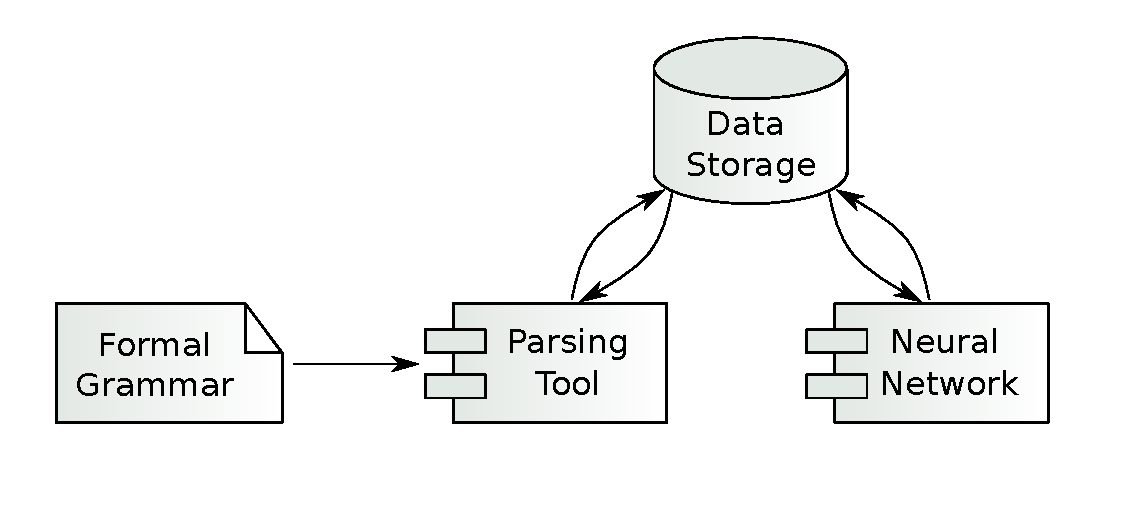
\includegraphics[width=12.0cm]{pics/diagram.pdf}
\caption{Архитектурные компоненты предложенного подхода}
\label{diagram}
\end{center}
\end{figure} 

Одной из потенциальных областей применения такого подхода является биоинформатика, в частности, различные задачи анализа РНК, где в качестве символьных последовательностей можно рассмотреть нуклеотидные цепочки РНК различных организмов, а в качестве синтаксической структуры --- биологическую вторичную структуру молекулы РНК. В текущей работе исследуется возможность применения описанного выше подхода для решения задачи предсказания вторичной структуры РНК. Далее будет описана разработанная для этого архитектура решения, включающая в себя два основных шага: задание грамматики для поиска характерных элементов вторичной структуры, а затем -- проектирование и обучение нейронных сетей, генерирующих для последовательности РНК максимально близкую к реальной вторичную структуру на основе полученных с помощью парсера данных.

\subsection{Формальная грамматика}
Первичная структура молекулы РНК представляет собой цепочку из нуклеотидов четырех типов (аденин, цитозин, гуанин и урацил), что в терминах синтаксического анализа есть последовательность символов алфавита \{A, C, G, U\}; вторичная же структура образовывается вследствие того, что некоторые участки первичной соединяются между собой, формируя рекурсивную композицию из шпилек разного размера и степени вложенности. Обобщенный вид таких шпилек может быть формализован средствами достаточно простой контекстно-свободной грамматики, каковой является используемая в данной работе грамматика $G_0$ (рис.~\ref{gram}). Грамматика учитывает только Уотсон-Криковские правила формирования нуклеотидных пар $A-U$, $C-G$ (строка \textbf{5}) и описывает рекурсивные композиции шпилек высоты от трех и более (строки \textbf{7-12}). Размер петли внутри шпильки лежит в пределах от одного до двадцати нуклеотидов, и такую же длину имеют последовательности, расположенные между любыми двумя шпильками (строка \textbf{2}). Эти числа были выбраны путем балансирования между следующими двумя соображениями: соответствие эмпирическим наблюдениям биологических данных и адекватность напрямую зависящих от длины и сложности грамматики временных затрат на работу парсера. По тем же причинам в $G_0$ не были включены неканонические нуклеотидные связи, которые могут встречаться в реальной вторичной структуре РНК --- для того, чтобы учесть все возможные пары нуклеотидов, придется ввести большое количество правил, имеющих вероятностную природу. Кроме того, средствами контекстно-свободных грамматик невыразимы псевдоузлы, однако псевдоузел есть комбинация из двух шпилек, следовательно, $G_0$, не описывая псевдоузел как единое целое, позволяет, тем не менее, выделить из входной последовательности обе составляющие его подстроки. Здесь становится понятным основное отличие нашего подхода от классического использования формальных грамматик в данной области~\cite{knudsen1999rna,dowell2004evaluation,rivas2000language} --- мы не пытаемся ни смоделировать вторичную структуру целиком, ни описать все возможные закономерности ее образования, но разбиваем ее на простые составные части, синтезировать из которых более сложные объекты предлагается уже с помощью нейронных сетей, что кратно уменьшает интеллектуальные и вычислительные затраты на синтаксический анализ.

\begin{figure}[h]
\begin{Verbatim}[numbers=left,xleftmargin=5mm]
s1: stem<s0>
any_str : any_smb*[1..20]
s0: any_str | any_str stem<s0> s0
any_smb: A | U | C | G
stem1<s>: A s U | G s C | U s A | C s G 
stem2<s>: stem1< stem1<s> >
stem<s>:  
      A stem<s> U 
    | U stem<s> A 
    | C stem<s> G 
    | G stem<s> C 
    | stem1< stem2<s> >  
\end{Verbatim}
\caption{Контекстно-свободная грамматика $G_0$ для описания шпилек вторичной структуры РНК}
\label{gram}
\end{figure}

Рассмотрим теперь формальный вид и практический смысл результата работы синтаксического анализатора для вышеописанной грамматики и последовательности РНК некоторого организма. Синтаксический анализ в данном случае используется для поиска всех подстрок входной строки, выводимых из стартового нетерминала $s1$ грамматики $G_0$, иными словами, для поиска тех участков этой строки, которые, в терминах $G_0$, могут свернуться в шпильки при формировании вторичной структуры. Формально, для входной строки $w$ парсер заполнит верхнетреугольную булеву матрицу --- матрицу разбора $M_P$, где $M_P[i,j]=1 \iff$ подстрока $w[i..j]$ выводится в $G_0$. Так как интересующие нас шпильки должны иметь высоту от трех, каждой шпильке высоты $n$ в матрице разбора будет соответствовать цепочка из $n - 2$ единиц. На рис.~\ref{mtrx} представлен результат работы парсера для изображенного на рис.~\ref{rna_a} случая последовательности, сворачивающейся в шпильку высоты четыре. Каждой нуклеотидной связи, образующей шпильку высоты от трех (сплошные линии голубого цвета), соответствует единица в ячейке матрицы разбора, при этом очевидно, что шпилька высоты три инкапсулирует в себе шпильки высоты два и один, обозначенные на рисунке пунктирными линиями. Помимо уже знакомой нам шпильки с рис.~\ref{rna_a}, в данной строке парсер обнаружил еще одну выводимую в грамматике подстроку (единица в позиции $[0,11]$): таким образом, для рассматриваемой цепочки существует два теоретически возможных варианта свертки, из которых реализованным на практике оказался только один.

\begin{figure}[h]
\begin{center}
\centering
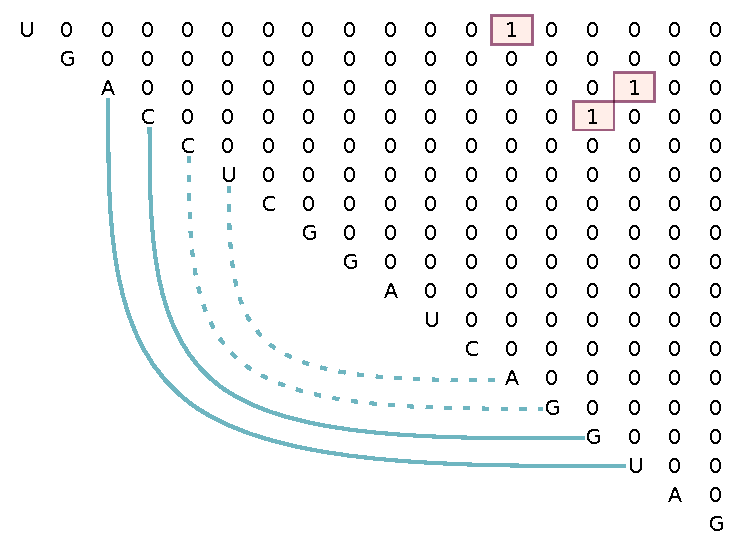
\includegraphics[width=10.0cm]{pics/matrix.pdf}
\caption{Матрица разбора для последовательности РНК}
\label{mtrx}
\end{center}
\end{figure} 
\vspace{3mm}

Остановимся в контексте предложенного подхода на проблеме обработки псевдоузлов, которые, как уже упоминалось ранее, не выводимы в используемой грамматике $G_0$. На рис.~\ref{pk_a} представлен пример последовательности, сворачивающейся в псевдоузел, а на рис.~\ref{pk_b} --- соответствующая данной последовательности матрица разбора. Рассматриваемый псевдоузел состоит из двух взаимопересекающихся шпилек высоты три и четыре, каждая из которых по отдельности выводима в $G_0$ и, следовательно, будет отражена в матрице разбора одной и двумя единицами соответственно. Несмотря на то, что на этапе синтаксического анализа еще не известно, образуют ли эти две найденные шпильки псевдоузел или же являются просто двумя теоретически возможными вариантами свертки цепочки, для нашего подхода предсказание псевдоузлов не становится ни сложностью, ни ограничением, так как матрицы разбора содержат всю необходимую о них информацию, которая должна быть более четко интерпретирована уже на этапе анализа данных нейронными сетями.

\captionsetup[subfigure]{justification=centering}
\begin{figure}[h]
\centering
\begin{subfigure}{.3\textwidth}
  \centering
  \fbox{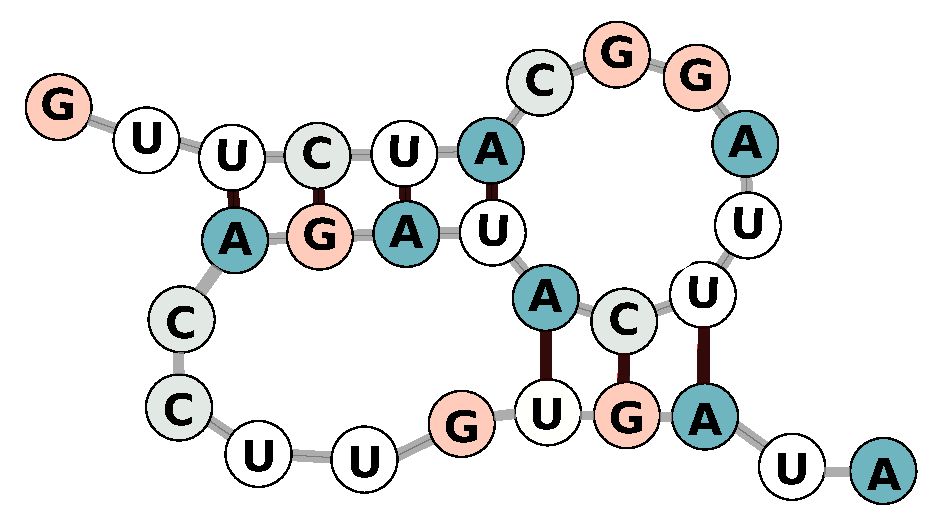
\includegraphics[width=.9\linewidth]{pics/pk.pdf}}
  \caption{Псевдоузел}
  \label{pk_a}
\end{subfigure}%
\begin{subfigure}{.7\textwidth}
  \centering
  \fbox{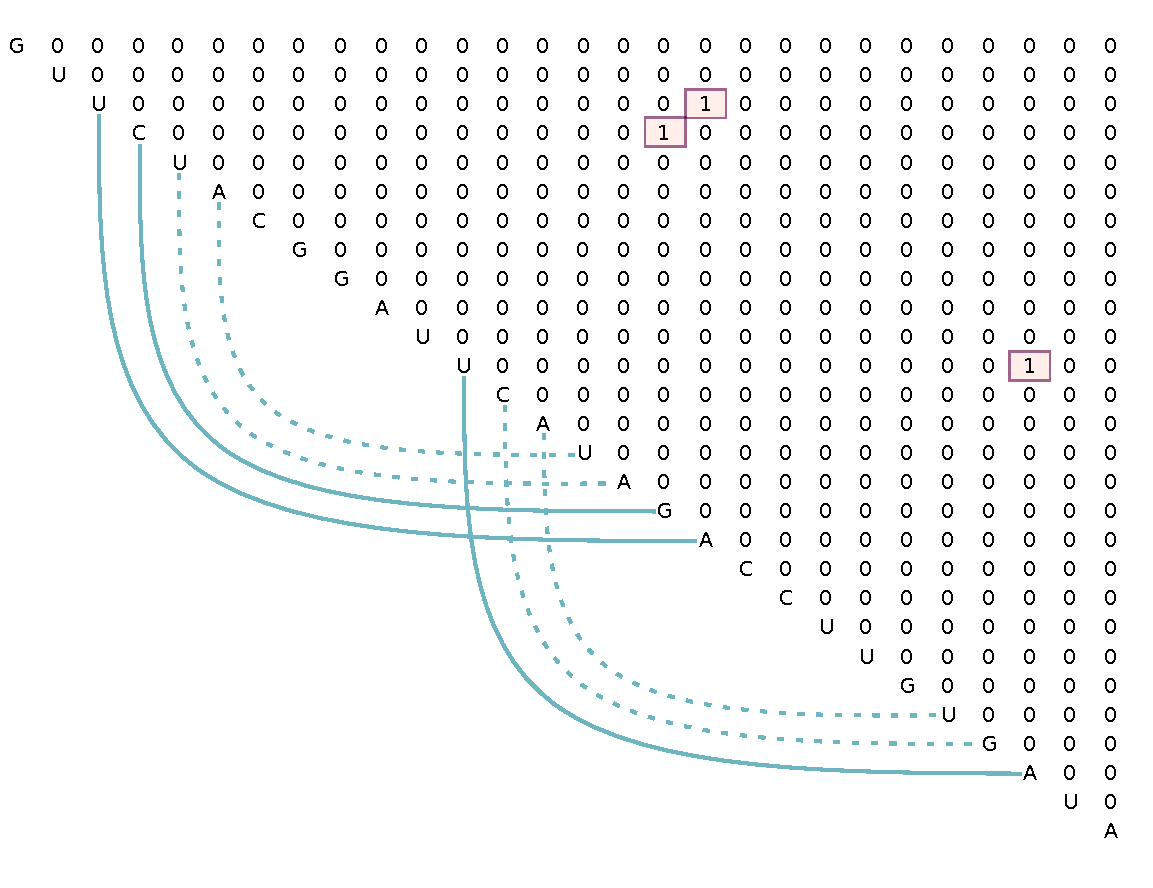
\includegraphics[width=.9\linewidth]{pics/matrix2.pdf}}
  \caption{Матрица разбора для последовательности с псевдоузлом}
  \label{pk_b}
\end{subfigure}
\caption{Обработка псевдоузлов в рамках предложенного подхода}
\label{pk}
\end{figure}

Таким образом, матрицы разбора хранят информацию о всех возможных расположениях шпилек вторичной структуры во входных последовательностях, однако на данный момент это только теоретические, искусственные объекты, для соотнесения которых с реальными биологическими данными требуется последующая обработка, и об этом будет подробно рассказано в следующем разделе.

\subsection{Нейронная сеть}
На данном этапе поставленная задача конкретизируется до следующей --- разработать нейронную сеть, которая принимает на вход матрицы, полученные синтаксическим анализатором по грамматике $G_0$ для некоторого набора последовательностей РНК, и, обучаясь на вторичных структурах, предоставленных в качестве эталонных для рассматриваемых последовательностей, оптимизирует параметры для преобразования матриц разбора в корректные вторичные структуры. Данный раздел посвящен описанию всех тонкостей этого процесса. 

\subsubsection{Подготовка данных} 
Входные данные для нейросети (матрицы разбора) были описаны в прошлом разделе, и теперь необходимо определить источник и формат эталонных данных. Существуют специализированные биологические базы данных, в которых размещены цепочки РНК различных организмов вместе с их извлеченными из природного материала или же полученными надежными методами вторичными структурами. Такие данные оптимальны для валидации, а, следовательно, и для обучения предсказывающих вторичную структуру алгоритмов. 

Как правило, в базах данных вторичные структуры РНК хранятся в скобочной (dot-bracket) нотации, из которой легко получить еще один классический формат  представления вторичной структуры --- так называемую матрицу контактов (contact map). Матрица контактов описывает наличие или отсутствие связи между каждыми двумя нуклеотидами последовательности: формально, для строки $w$ это верхнетреугольная булева матрица $M_C$, где $M_C[i,j]=1 \iff w[i]$ и $w[j]$ образуют пару во вторичной структуре. Как было описано в прошлом разделе, результат работы парсера на входной строке $w$ --- верхнетреугольная булева матрица $M_P$, где $M_P[i,j]=1 \iff w[i..j]$ свернется в шпильку по правилам грамматики. Нетрудно проверить, что наличие контакта между нуклеотидами $w[i]$ и $w[j]$ эквивалентно тому факту, что последовательность $w[i..j]$ является шпилькой, поэтому, несмотря на то, что наше определение вторичной структуры как композиции вложенных шпилек не относится к общеупотребимым, матрицу разбора можно также описать как матрицу контактов, формируемых только выразимыми в грамматике элементами. Таким образом, использование матричного представления вторичной структуры при подготовке эталонных данных для нейронной сети представляется самым удобным в свете специфики используемых в качестве входных данных матриц разбора. 

Для наглядности и удобства применения нейронных сетей мы предлагаем смотреть на матрицу контактов и матрицу разбора как на изображения: пикселями белого цвета обозначим позиции в матрицах с единицами, черного --- с нулями. Матрицы разбора содержат $n - 2$ единицы для каждой шпильки высоты $n>3$, следовательно, в качестве предобработки перед обучением нейросети для каждой единицы в матрице разбора следует добавить еще две единицы в направлении главной диагонали. Кроме того, сама нуклеотидная последовательность РНК может содержать некоторую важную информацию, поэтому предлагается закодировать ее на главной диагонали изображений равноотстающими друг от друга серыми пикселями. 

На рисунке~\ref{struc} продемонстрировано, как для одной и той же последовательности РНК будут выглядеть входной и эталонный образцы для нейронной сети, а также показана визуализация соответствующей вторичной структуры. Контакты, относящиеся к трем присутствующим в рассматриваемой цепочке шпилькам, на всех изображениях выделены голубым, сиреневым и розовым цветами. Данный рисунок является наглядным примером того, что далеко не все найденные парсером шпильки будут представлены в реальной вторичной структуре (белые пиксели изображения~\ref{struc_c}). Кроме того, видно, что в сгенерированной синтаксическим анализатором матрице отсутствует несколько эталонных контактов: в данном случае это произошло из-за того, что они были образованы непредусмотренными грамматикой неканоническими нуклеотидными парами. 

\captionsetup[subfigure]{justification=centering}
\begin{figure}[h]
\centering
\begin{subfigure}{.3\textwidth}
  \centering
  \fbox{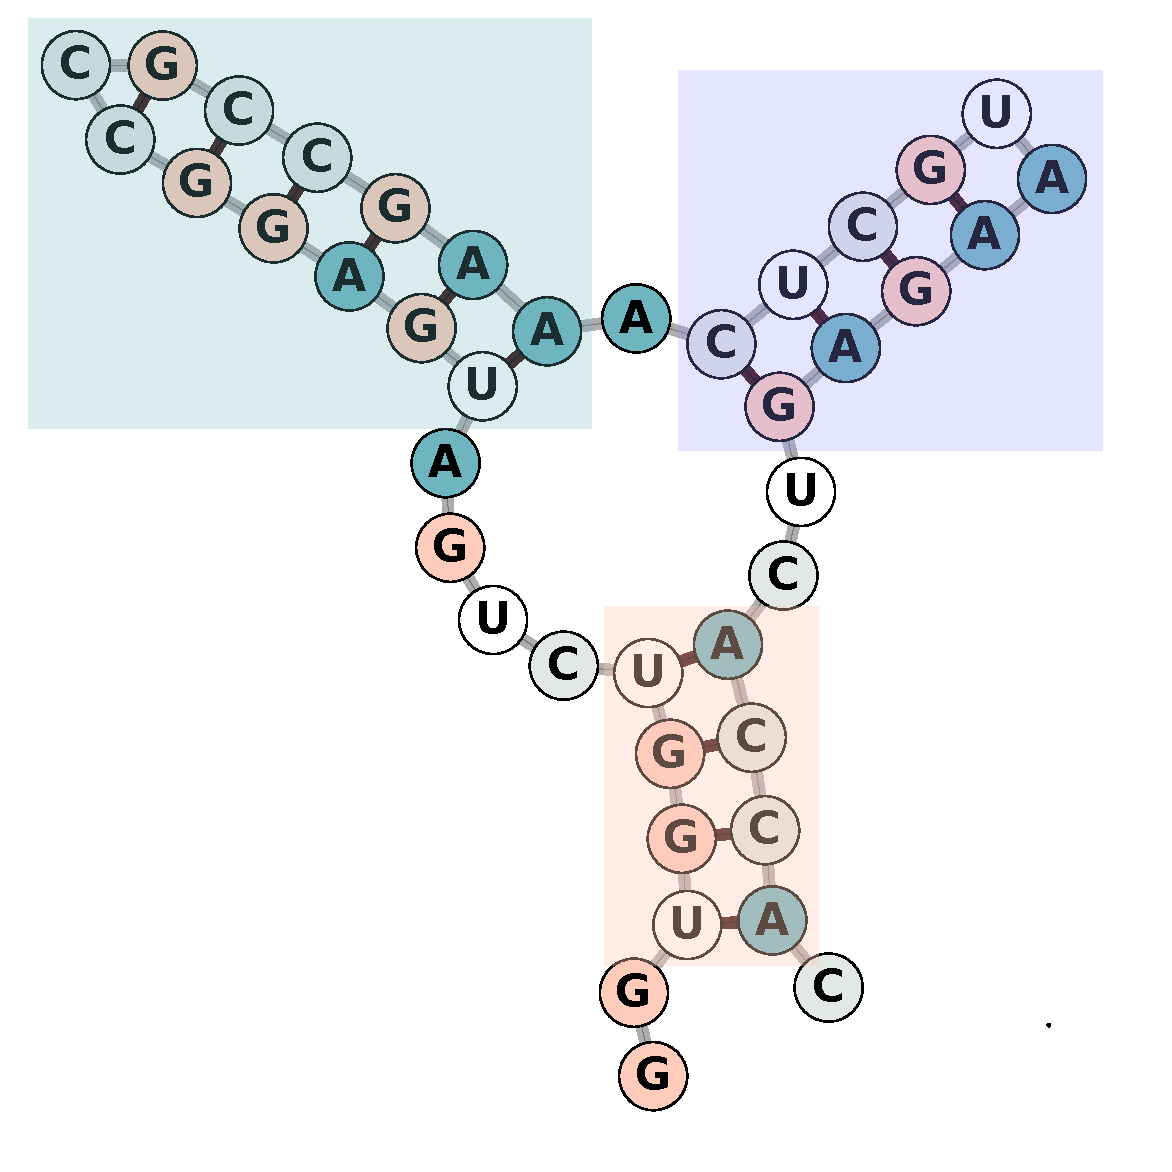
\includegraphics[width=.9\linewidth]{pics/struct.pdf}}
  \caption{Визуализация вторичной структуры}
  \label{struc_a}
\end{subfigure}%
\begin{subfigure}{.3\textwidth}
  \centering
  \fbox{
\includegraphics[width=.9\linewidth]{pics/out.png}}
  \caption{Эталонный  образец \\ для нейросети}
  \label{struc_b}
\end{subfigure}
\begin{subfigure}{.3\textwidth}
  \centering
  \fbox{
\includegraphics[width=.9\linewidth]{pics/in.png}}
  \caption{Входной образец \\ для нейросети}
  \label{struc_c}
\end{subfigure}
\caption{Примеры представления вторичной структуры}
\label{struc}
\end{figure}

Таким образом, в рамках данного исследования перед нейронной сетью стоит задача отфильтровать и дополнить матрицу разбора, сгенерировав корректную матрицу контактов, соответствующую максимально близкой к эталонной вторичной структуре.

\subsubsection{Параллельная остаточная архитектура}
Рассмотрим общую модель нейронной сети, разработанной в рамках данной работы. Входными и выходными данными являются изображения, и для решения поставленной задачи необходимо найти достаточно сложные закономерности между элементами данных, находящимися на большом расстоянии друг от друга, поэтому была использована глубокая сверточная сеть. Для оптимизации процесса обучения и повышения скорости сходимости была применена технология остаточных нейронных сетей. В процессе экспериментальных исследований нами было выявлено, что точность результатов значительно повышает использование $n$ остаточных сетей с одинаковой архитектурой, которые обучаются параллельно на одних и тех же данных, находя в них, по всей видимости, немного разные паттерны, а затем соединяются слоем, подсчитывающим линейную комбинацию их $n$ выходов и передающим ее уже общему остаточному блоку, завершающему обработку данных. Такая новая параллельная архитектура представлена на рис.~\ref{nn}; там же показано, как выглядит типичный остаточный блок (residual unit) нейронной сети, состоящий из пяти сверточных слоев с постепенно убывающими количеством фильтров и размером ядра свертки. В данной работе была использована модель, состоящая из четырех остаточных сетей с пятью одинаковыми блоками в каждой.

\begin{figure}[h]
\begin{center}
\centering
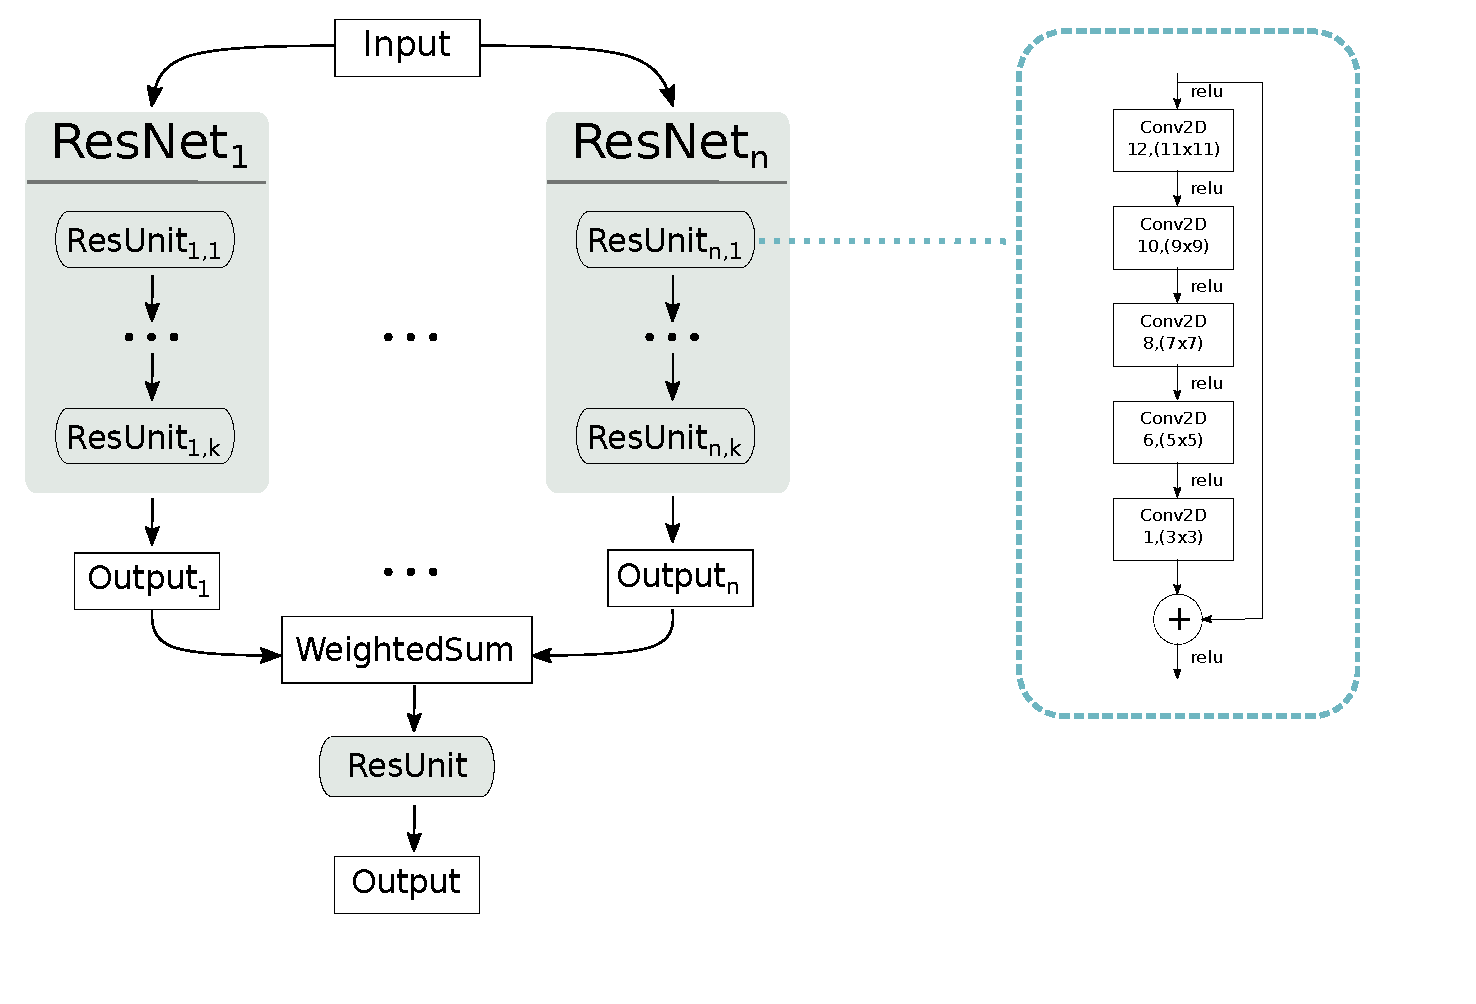
\includegraphics[width=15cm]{pics/nn.pdf}
\caption{Параллельная остаточная нейронная сеть}
\label{nn}
\end{center}
\end{figure} 

\section{Эксперименты}
This section demonstrates the practical results of the proposed approach application. We introduce an easy-to-use implementation, specify some experimental details and describe currently available models. We compare our results with several popular tools and show the competitive power of our models.

\subsection{Tool}
The proposed approach was implemented as a Python console tool Genegram. Code, installation instructions, and documentation are available by link \linebreak \url{https://github.com/JetBrains-Research/Genegram}. This tool accepts a file with RNA sequences in fasta format and returns the connectivity tables (ct) for the corresponding secondary structures. We use an effective Python implementation of the parsing algorithm~\cite{Azimov:2018:CPQ:3210259.3210264} that shows high performance due to the GPGPU utilization and Keras~\cite{chollet2015keras} library with Tensorflow-GPU~\cite{tensorflow2015-whitepaper} framework for running the predictive model. Genegram tool allows to select different models and process sequences of lengths 1-200 containing only four canonical nucleotides.

\subsection{Setup}
The approach itself is quite flexible and Genegram tool provides a convenient environment for different experiments allowing to change both grammar and network. However, in the present work, we freeze grammar $G_0$ from figure~\ref{gram} and parallel ResNet architecture from figure~\ref{nn} with $k := 10$, $n := 4$. We consider only small RNAs (lengths from 1 to 200) due to the insufficient amount of longer sequences in biological databases and GPU storage limitations. Each sequence of $l$ nucleotides results in the image of size $l \times l$, therefore, images are grouped into batches by image size and cyclically duplicated until all batches have the same length. We use two data augmentation techniques on the training dataset: firstly, we mirror each image along the main diagonal (so that mirrored image represents the same sequence turned backwards), and secondly, we copy both regular and mirrored images twice. On this data, we run 10-fold cross-validation in order to choose the best train and validation split for each model.

The quality of the results is estimated by classical machine learning metrics calculated on the pixel-by-pixel difference between predicted and reference images. Further, we consider $TP$ (true positives, i.e. true white pixels), $FP$ (false positives, i.e. false white pixels), and $FN$ (false negatives, i.e. false black pixels) as numbers of right and wrong decisions among all contacts and calculate three following metrics for each image of some dataset. 

\begin{itemize} 
    \item $Precision = \displaystyle \frac{TP}{TP + FP}$ (proportion of correct contacts among all detected).
    \item $Recall = \displaystyle \frac{TP}{TP + FN}$ (proportion of detected contacts among all expected).
    \item $F1 = \displaystyle 2 * \frac{Precision * Recall}{Precision + Recall}$ (harmonic mean --- aggregation metrics).
\end{itemize}

The loss function is based on the idea of maximizing $F1$ score and that is to be achieved by minimizing the dataset mean $1 - F1$ through gradient descent. However, $F1$ is not differentiable as a function, so, we replace the sums of discrete integer values with a continuous sum of probabilities. Also, we charge our loss with two penalty coefficients responsible for huge dispersion between $Precision$ and $Recall$ for each image ($k1$) and the whole dataset ($k2$). Figure~\ref{loss} demonstrates the Python code for the currently used  $F1\_loss$ function that accepts two arguments: predicted image $y\_p$ and true image $y\_t$.

\begin{figure}[h]
\centering
\begin{lstlisting}[language=Python]
from keras import backend as K

def f1_loss(y_t, y_p):
    #normalize pixels values to [0, 1]
    y_t, y_p = K.minimum(y_t / 255, 1), K.minimum(y_p / 255, 1)
    #calculate differentiable versions of tw, fw and fb
    tw = K.sum(K.cast(y_t * y_p, 'float32'), axis=[1, 2, 3])
    fw = K.sum(K.cast((1 - y_t) * y_p, 'float32'), axis=[1, 2, 3])
    fb = K.sum(K.cast(y_t * (1 - y_p), 'float32'), axis=[1, 2, 3])
    #calculate precision and recall secure from zero division error
    prec = tw / (tw + fw + K.epsilon())
    rec = tw / (tw + fb + K.epsilon())
    #penalties for huge difference between precision and recall 
    #calculated for each image and whole dataset respectively
    k1 = 1 -  K.abs(prec- rec)
    k2 = 1 -  K.abs(K.mean(prec) - K.mean(rec))
    #calculate upgraded f1 score and return its mean value
    f1 = k1 * k2 * 2 * prec * rec / (prec + rec + K.epsilon()) 
    return 1 - K.mean(f1)
\end{lstlisting}
\caption{$F1\_loss$ function}
\label{loss}
\end{figure} 

For hyperparameters, we use Dropout after each residual unit to deal with overfitting, L2-regularization that also prevents overfitting and allows to search for complex data patterns, and Adagrad optimizer that automatically sets the learning rate and is known to be a powerful solution for sparse data processing.

For a comparative analysis of the results we selected six tools based on various concepts and algorithms. All of them demonstrate adequate speed and high accuracy, can handle pseudoknots and are easy to launch and use.

\begin{itemize}
    \item SPOT-RNA~\cite{singh2019rna} --- deep neural networks + transfer learning.
    \item Ipknot~\cite{sato2011ipknot} --- MEA + integer programming.
    \item Knotty~\cite{jabbari2018knotty} --- MFE + sparse dynamic programming.
    \item RNAstructure~\cite{bellaousov2013rnastructure} --- MFE + dynamic programming. 
    \item PknotsRG~\cite{reeder2007pknotsrg} --- MFE + Turner energy rules.
    \item HotKnots~\cite{ren2005hotknots} --- MFE + heuristic algorithm.
\end{itemize}

\subsection{Models}
In these conditions, we trained three identical networks on three different datasets and compared them with each other and with other tools by several criteria. All three models are available to use in the Genegram tool and the default model here is Genegram-main. Let us describe the specifics of each dataset, present the results of the best 10-fold cross-validation splits, and draw some conclusions.

\subsubsection{Genegram-main}
The first model was trained on data obtained from RNA STRAND database~\cite{andronescu2008rna} that is quite popular in different RNA analysis research due to its quality and usability. This database is an assembly of carefully curated and validated RNA sequences with secondary structures collected from different sources, and it contains only trustful structures obtained by reliable methods (laboratory or comparative). This database is supposed to provide the most representative sample of RNA secondary structures along with a guaranteed high quality of data which makes Genegram-main model trained on RNA STRAND the most general one for now, therefore, we set it as a default choice for our tool.

We selected 1091 sequences with lengths up to 200 and removed samples with gaps or inaccuracies in primary and secondary structures. The distribution of sequences lengths in the prepared dataset is demonstrated in figure~\ref{main_distr}. Neural network output images are grayscale and may contain multiple contacts, therefore, we applied binarization by threshold 0.6 with multiplets removal as postprocessing for this model and calculated the following metrics afterwards. Figure~\ref{main_f1} shows the estimation of Genegram-main and other six tools on validation set of size 109 by metrics $F1$. The shape of colored plots shows the density of $F1$ values, the red line represents its median result and the blue line corresponds to the mean one. It can be seen that Genegram-main has median $F1$ equal to 81 (as well as Knotty which is the second result after SPOT-RNA), and mean $F1$ equal to 70 that significantly exceeds the results of all competing tools except SPOT-RNA. The estimation on the same set by mean $Precision$ and $Recall$ metrics is presented in figure~\ref{main_pr}. Note that the binarization threshold allows us to slightly manipulate the balance between these two metrics and we choose it so that $F1$ mean value is the highest, even though it leads to a small excess of $Precision$ over $Recall$.

\begin{figure}[h]
\centering
    \subfloat[$F1$ distribution, mean, \\ and median on valid set]
        {\label{main_f1}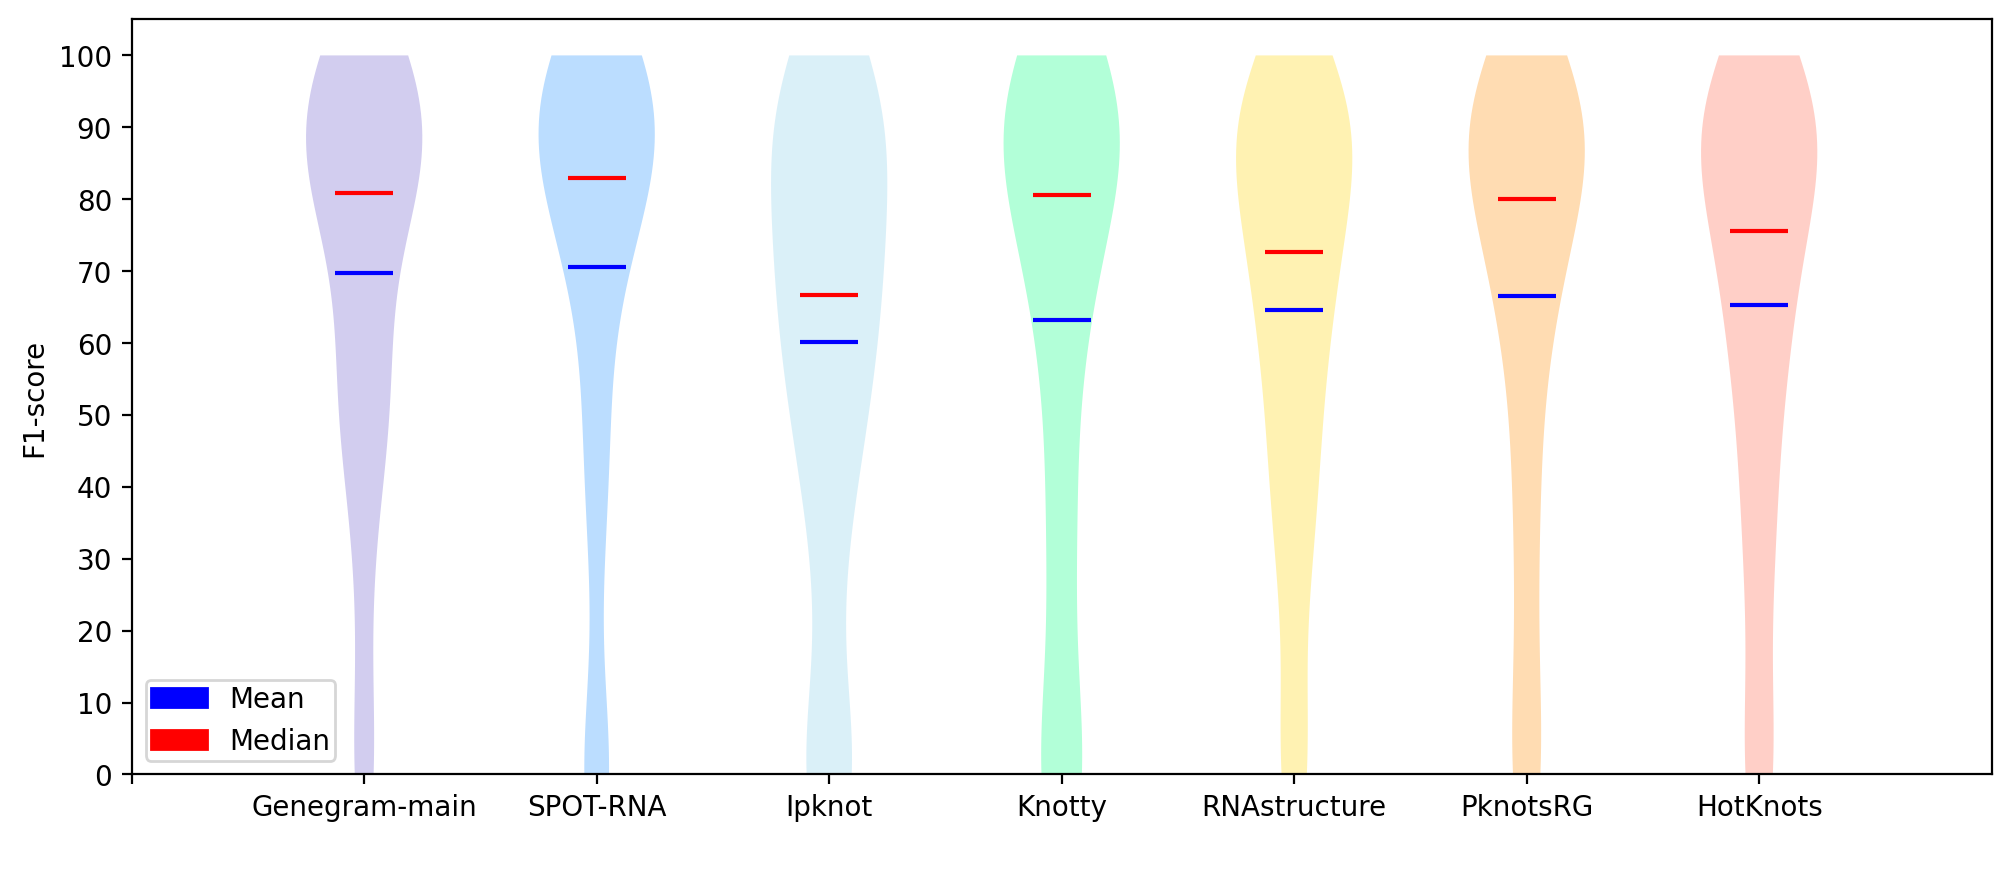
\includegraphics[width=.69\linewidth]{pics/plot_main_f1.png}}\hfill
    \subfloat[$Precision$ and $Recall$ mean on valid set]
        {\label{main_pr}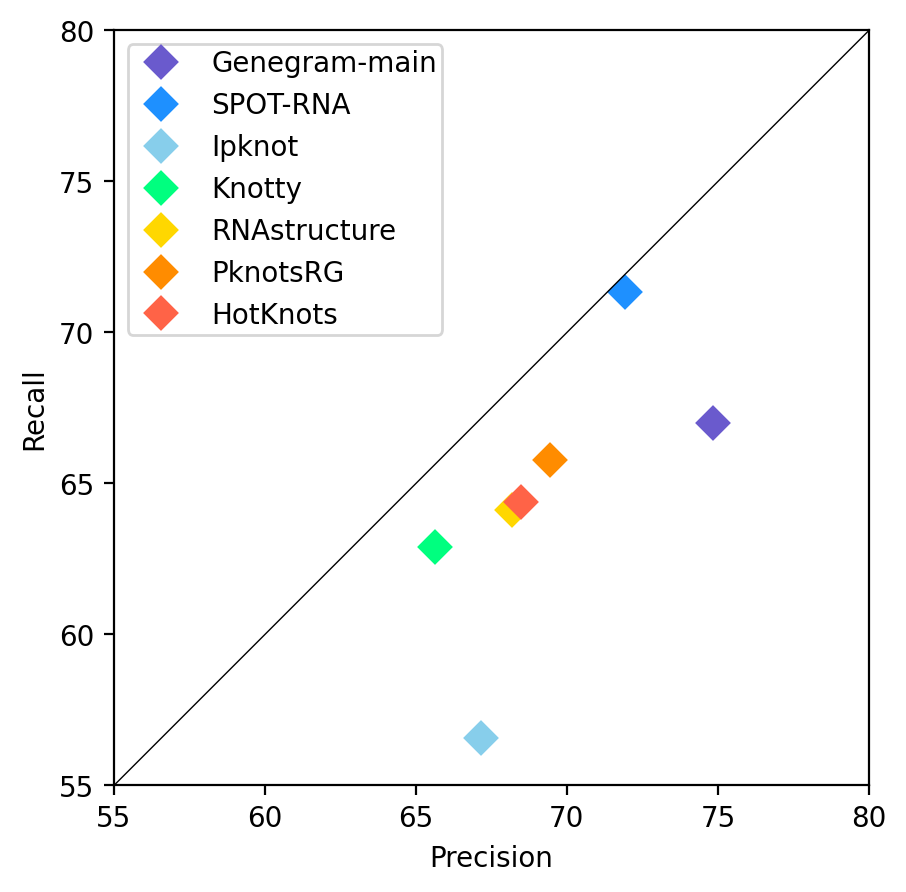
\includegraphics[width=.31\linewidth]{pics/plot_main_pr.png}}\par 
    \subfloat[Sequences lengths distribution on total set]
        {\label{main_distr}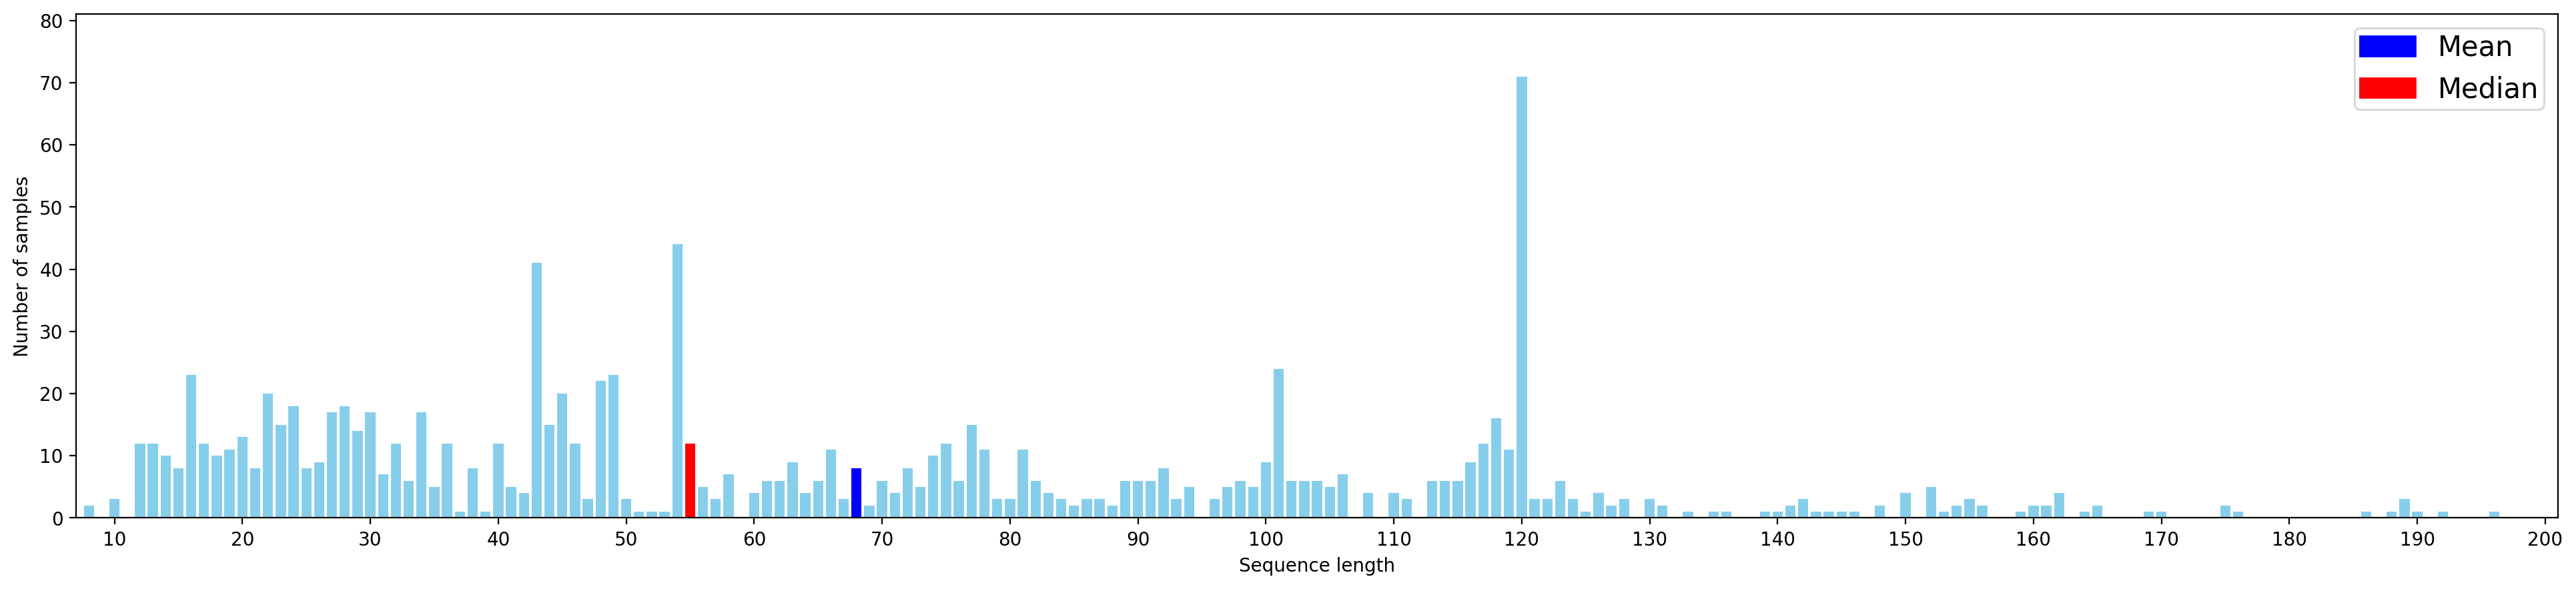
\includegraphics[width=\linewidth]{pics/plot_main_distr.png}}
\caption{Analysis of Genegram-main model compared with other tools }
\label{plots_main}
\end{figure}

All models were also estimated by several more specific functional criteria, such as pseudoknots prediction accuracy and sensitivity to different types of base pairs, so, table~\ref{table_main} demonstrates the results of these experiments. Considered validation set contained 11 pseudoknots and we calculated the number of correctly predicted contacts for each pseudoknot in each model output. The second column of table~\ref{table_main} shows the number of perfectly detected pseudoknots and the third column --- the number of ones that had up to 25\% extra or missing contacts. Clearly, pseudoknotted structures prediction is a non-trivial task for almost all models including Genegram-main. The other three columns of table~\ref{table_main} demonstrate how these tools handle different types of base pairs. Watson-Crick pairs are the most common and stable ones and it can be seen that all models have high enough canonical pairs prediction accuracy. Besides, it is known that wobble base pairs also have a biological role and regularly appear in real-world data, especially GU pair that has stability close to the Watson-Crick bonds. Our model slightly loses to other tools in GU pairs prediction, however, the great advantage of our approach is that it does not limit any types of pairs to be presented in neural network output (as well as SPOT-RNA that also uses neural networks), so, Genegram-main and SPOT-RNA are able to handle seven more wobble base pairs (AA, AC, AG, CC, CU, GG, UU), unlike other considered tools.

\begin{table}[h!]
\centering
\caption{Genegram-main and other models quality criteria measured on valid set}
\ra{1.4}
\begin{tabular}{@{}lccccccc@{}}\toprule
& \multicolumn{2}{c}{Pseudoknots} & \phantom{abc}& \multicolumn{3}{c}{Base pairs} \\
& No errors & 25\% errors  && Watson-Crick & GU & Others \\ \cmidrule{2-3} \cmidrule{5-7} 
Genegram-main  & 0 & 3 && 1067 & 68 & 53 \\
SPOT-RNA & 1 & 4 && 1190 & 134 & 39 \\
Ipknot & 0 & 1 && 939 & 92 & 0 \\
Knotty &1 & 3 && 1093 & 126 & 0 \\
RNAstructure & 1 & 1 && 1113 & 119 & 0 \\
PknotsRG & 1 & 5 && 1157 & 123 & 0 \\
HotKnots & 1 & 2 && 1113 & 112 & 0 \\
\bottomrule
Expected & 11 & 11 && 1650 & 185 & 135 \\
\bottomrule
\end{tabular}
\label{table_main}
\end{table}

\subsubsection{Genegram-pks}
Although the main model shows high results in general, it has poor pseudoknots prediction accuracy because RNA STRAND database contains only 86 sequences with pseudoknots and the neural network has not enough data to learn them, moreover, the amount of pseudoknots in the considered validation set is not enough to draw any conclusions. To improve this, we extended the previous dataset with sequences from Pseudobase~\cite{van2000pseudobase} database that is known to be a carefully built collection of pseudoknotted structures. Even though this database mostly contains not the whole sequences but only fragments with pseudoknots, we believe that the presence of such data in the training set may allow us to reach higher results in pseudoknots prediction.

We selected 1447 sequences having lengths up to 200 with no gaps or inaccuracies in primary and secondary structures and applied the same binarization by threshold 0.6 with multiplets removal as postprocessing. Note that both times we used 10-fold cross-validation on randomly shuffled data, so, Genegram-pks has separate from Genegram-main validation set, even though samples may intersect. Figure~\ref{pks_distr} shows the distribution of sequences lengths in total Genegram-pks dataset, figure~\ref{pks_f1} estimates all seven models on 145 validation sequences by $F1$ and figure~\ref{pks_pr} --- by $Precision$ and $Recall$ metrics. Genegram-pks is behind two tools by mean $F1$ value (70) and behind three tools by median (75) one, so, these results are quite competitive, however, Genegram-main was able to achieve the higher numbers.

\begin{figure}
\centering
    \subfloat[$F1$ distribution, mean, \\ and median on valid set]
        {\label{pks_f1}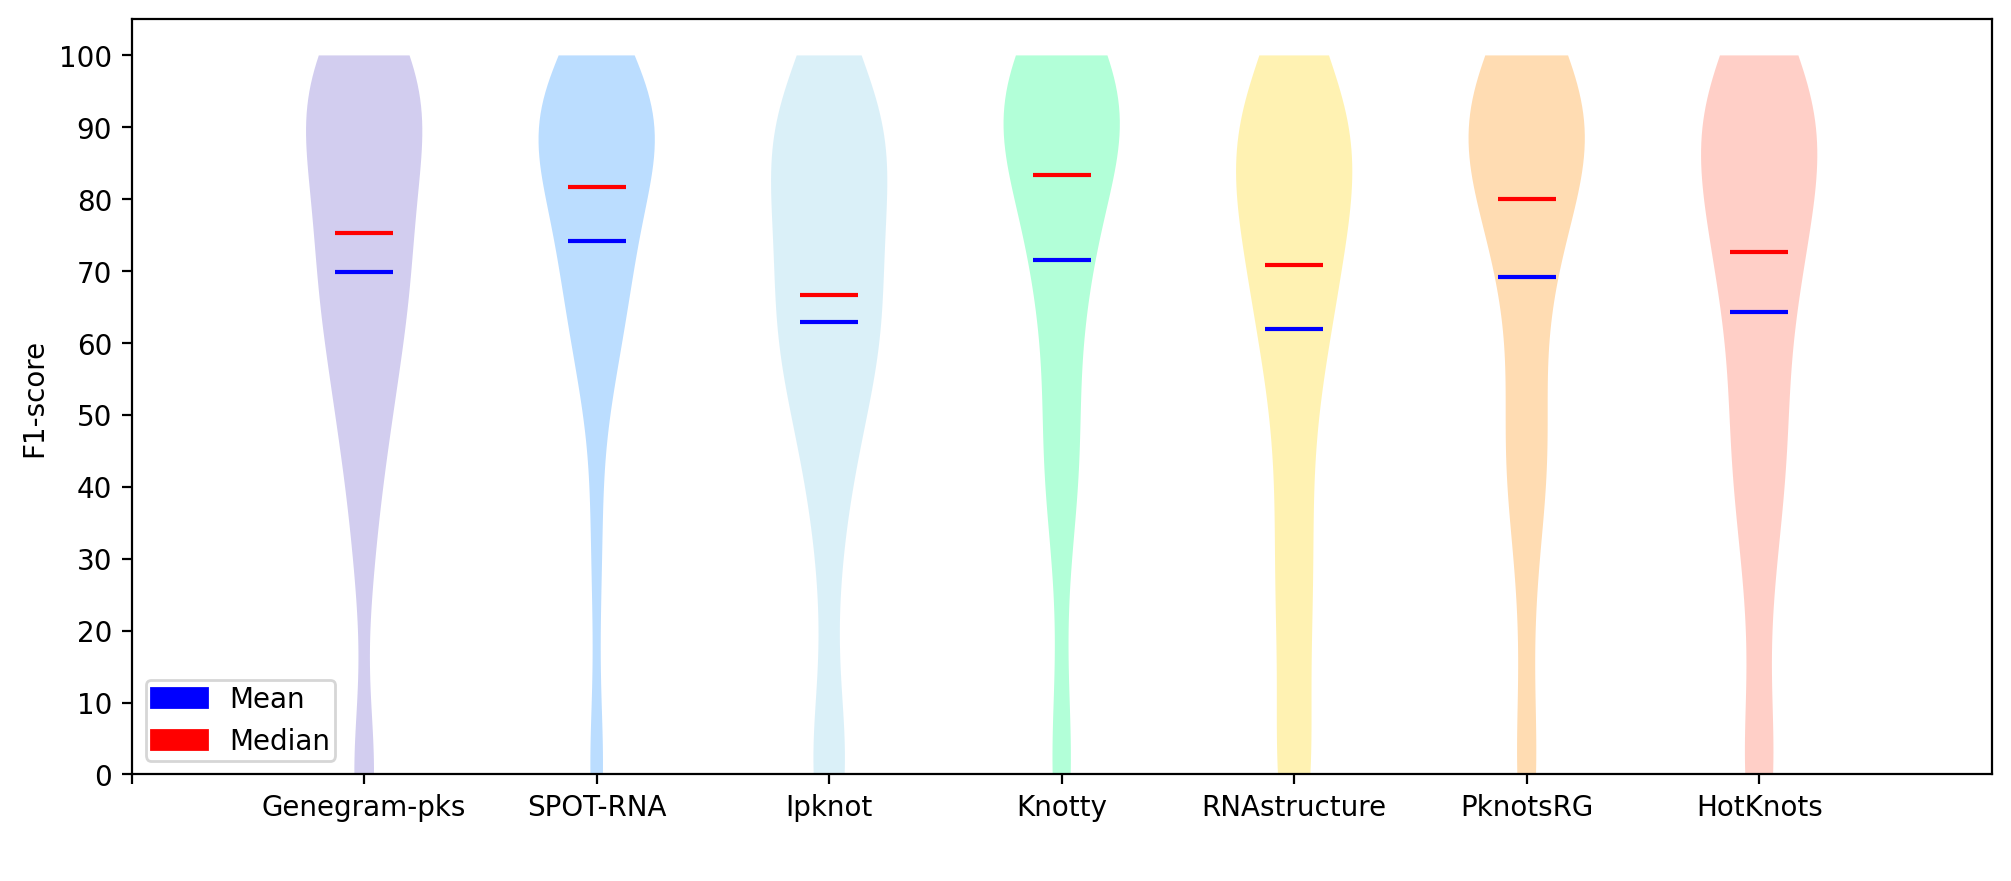
\includegraphics[width=.69\linewidth]{pics/plot_pks_f1.png}}\hfill
    \subfloat[$Precision$ and $Recall$ mean on valid set]
        {\label{pks_pr}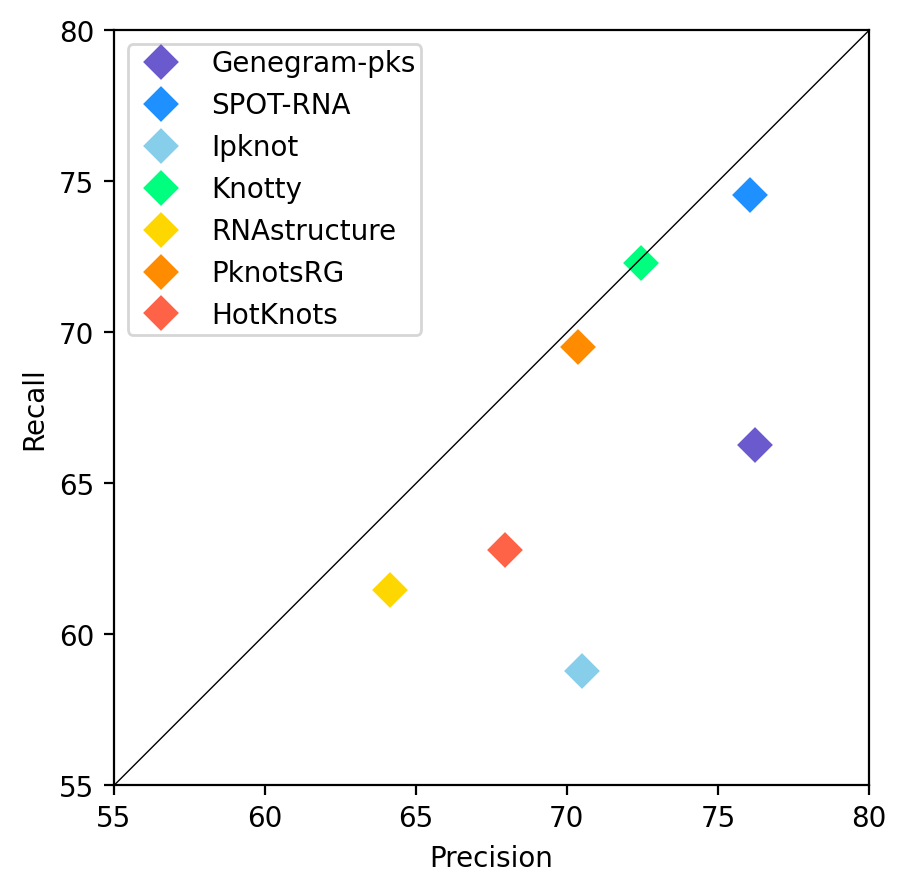
\includegraphics[width=.31\linewidth]{pics/plot_pks_pr.png}}\par 
    \subfloat[Sequences lengths distribution on total set]
        {\label{pks_distr}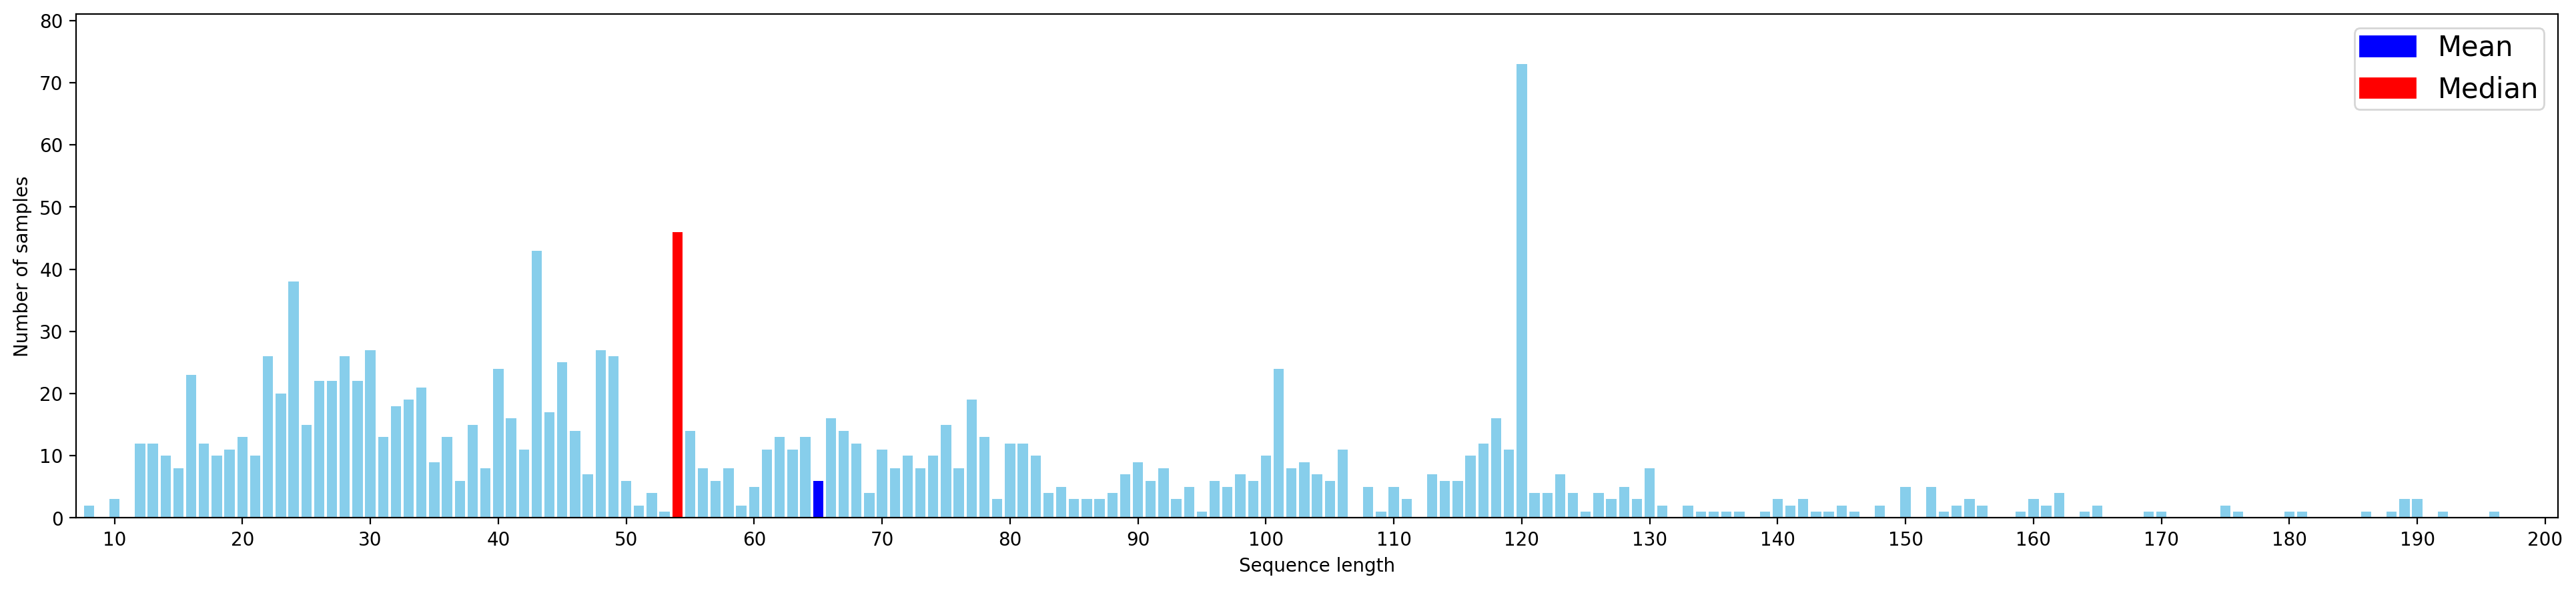
\includegraphics[width=\linewidth]{pics/plot_pks_distr.png}}
\caption{Analysis of Genegram-pks model compared with other tools }
\label{plots_pks}
\end{figure}

Similarly, we present the results of functional tests for this model and other tools in table~\ref{table_pks}. It can be seen that Watson-Crick pairs are predicted similarly to the main model, but wobble base pairs prediction accuracy decreased. However, the pseudoknotted structures processing was of particular interest in the context of Genegram-pks model and estimation by this criteria shows significant growth compared to the Genegram-main --- almost a quarter of all pseudoknots was detected perfectly, and about a half had small prediction errors. To sum up, this model generally losses to the main one, however, it shows very promising results in the aspect of pseudoknots detection being one of the best models for this problem.

\begin{table}
\centering
\caption{Genegram-pks and other models quality criteria measured on valid set}
\ra{1.4}
\begin{tabular}{@{}lccccccc@{}}\toprule
& \multicolumn{2}{c}{Pseudoknots} & \phantom{abc}& \multicolumn{3}{c}{Base pairs} \\
& No errors & 25\% errors  && Watson-Crick & GU & Others \\ \cmidrule{2-3} \cmidrule{5-7} 
Genegram-main  & 9 & 18 && 1628 & 61 & 47 \\
SPOT-RNA & 4 & 10 && 1893 & 173 & 71 \\
Ipknot & 2 & 5 && 1497 & 120 & 0 \\
Knotty & 11 & 20 && 1833 & 156 & 0 \\
RNAstructure & 3 & 7 && 1550 & 140 & 0 \\
PknotsRG & 11 & 20 && 1742 & 150 & 0 \\
HotKnots & 6 & 6 && 1621 & 143 & 0 \\
\bottomrule
Expected & 43 & 43 && 2407 & 258 & 156 \\
\bottomrule
\end{tabular}
\label{table_pks}
\end{table}

\subsubsection{Genegram-mps}
Another object that our approach allows to consider without any explicit definition is a multiplet that appears when base pair starts to form bonds with other bases or base pairs producing various topologies~\cite{bhattacharya2019going}. Multiplets are known to be functionally important, although, they are classified as tertiary structure features, so, secondary structure prediction tools are not usually able to handle them. In our terminology, multiplet would result in a reference image containing a set of white pixels where every two pixels have one equal coordinate, which makes multiplets processing possible in the terms of the considered approach.

For this experiment, we used data from PDB database~\cite{berman2000protein} that includes extracted from natural material RNA molecules with the corresponding crystallography results providing detailed structural information about secondary and tertiary interactions. This data tends to contain a lot of variability and complicated patterns, therefore, it creates more research possibilities but also makes it harder to learn. So, Genegram-mps is a network that was trained on data from the PDB database and for now, it is an experimental model that has possibilities in predicting more features, especially, multiplets. We selected 712 sequences with lengths up to 200 and kept samples with interactions with other molecules and up to 20\% unmodeled residues due to the insufficient amount of perfectly clean samples in this database. We used RNAView software~\cite{yang2003tools} to generate base pairs list from RNA crystallography files and extended $F1\_loss$ function with a penalty coefficient that considers the percentage of correctly predicted multiplets contacts in all images. Also, we applied a smaller binarization threshold of 0.45 for this model. Figure~\ref{mps_distr} demonstrates the distribution of sequences lengths in the whole dataset, figure~\ref{mps_f1} estimates all models on 71 validation sequences by $F1$ metrics and figure~\ref{mps_pr} --- by $Precision$ and $Recall$ metrics. Genegram-mps has a slightly lower $F1$ value than other tools, however, it shows the highest $Recall$ due to the fact that it is the only model that can predict multiplets. 

\begin{figure}
\centering
    \subfloat[$F1$ distribution, mean, \\ and median on valid set]
        {\label{mps_f1}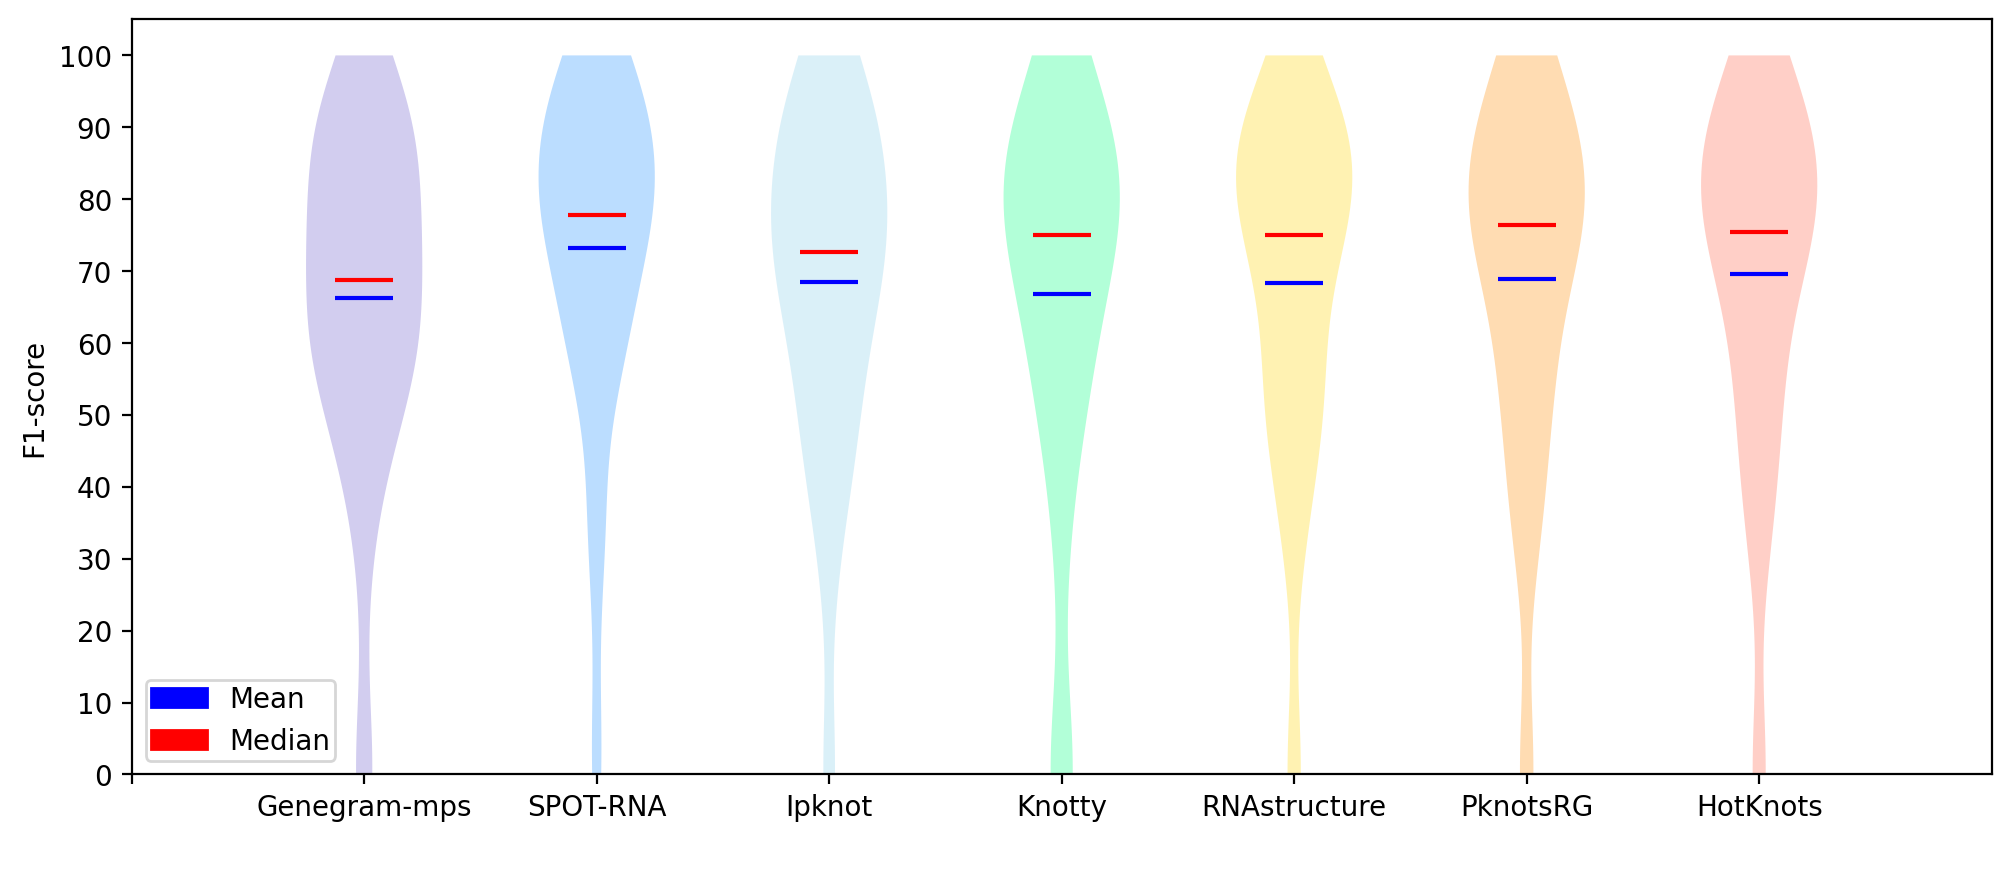
\includegraphics[width=.69\linewidth]{pics/plot_mps_f1.png}}\hfill
    \subfloat[$Precision$ and $Recall$ mean on valid set]
        {\label{mps_pr}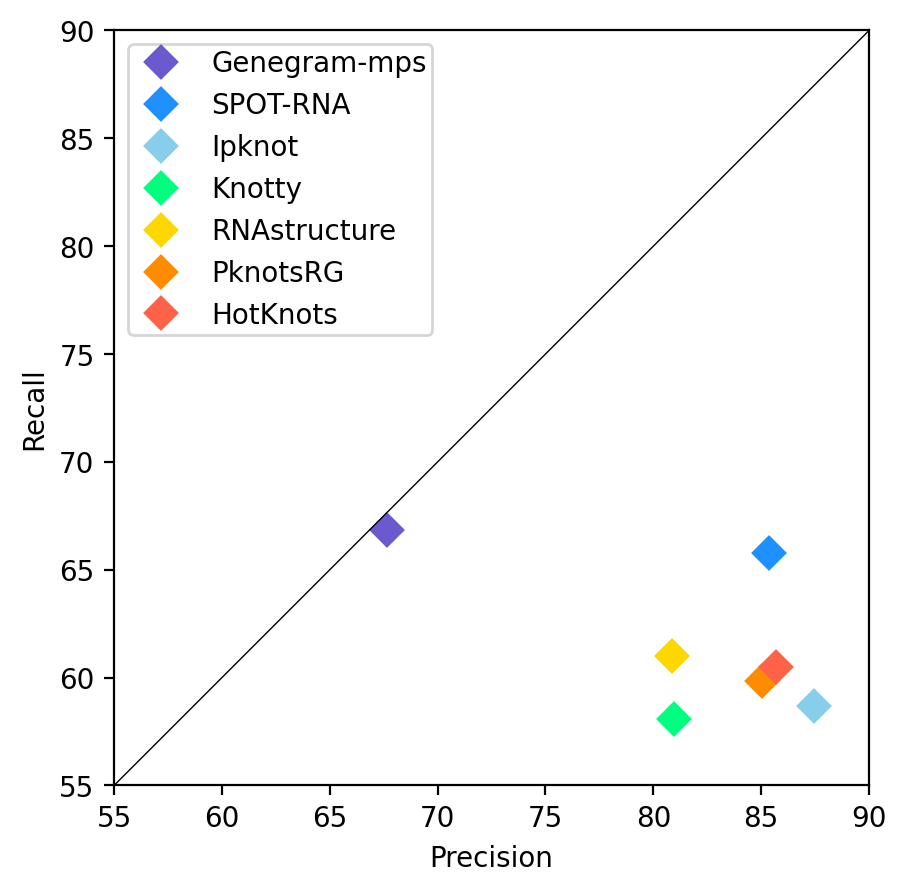
\includegraphics[width=.31\linewidth]{pics/plot_mps_pr.png}}\par 
    \subfloat[Sequences lengths distribution on total set]
        {\label{mps_distr}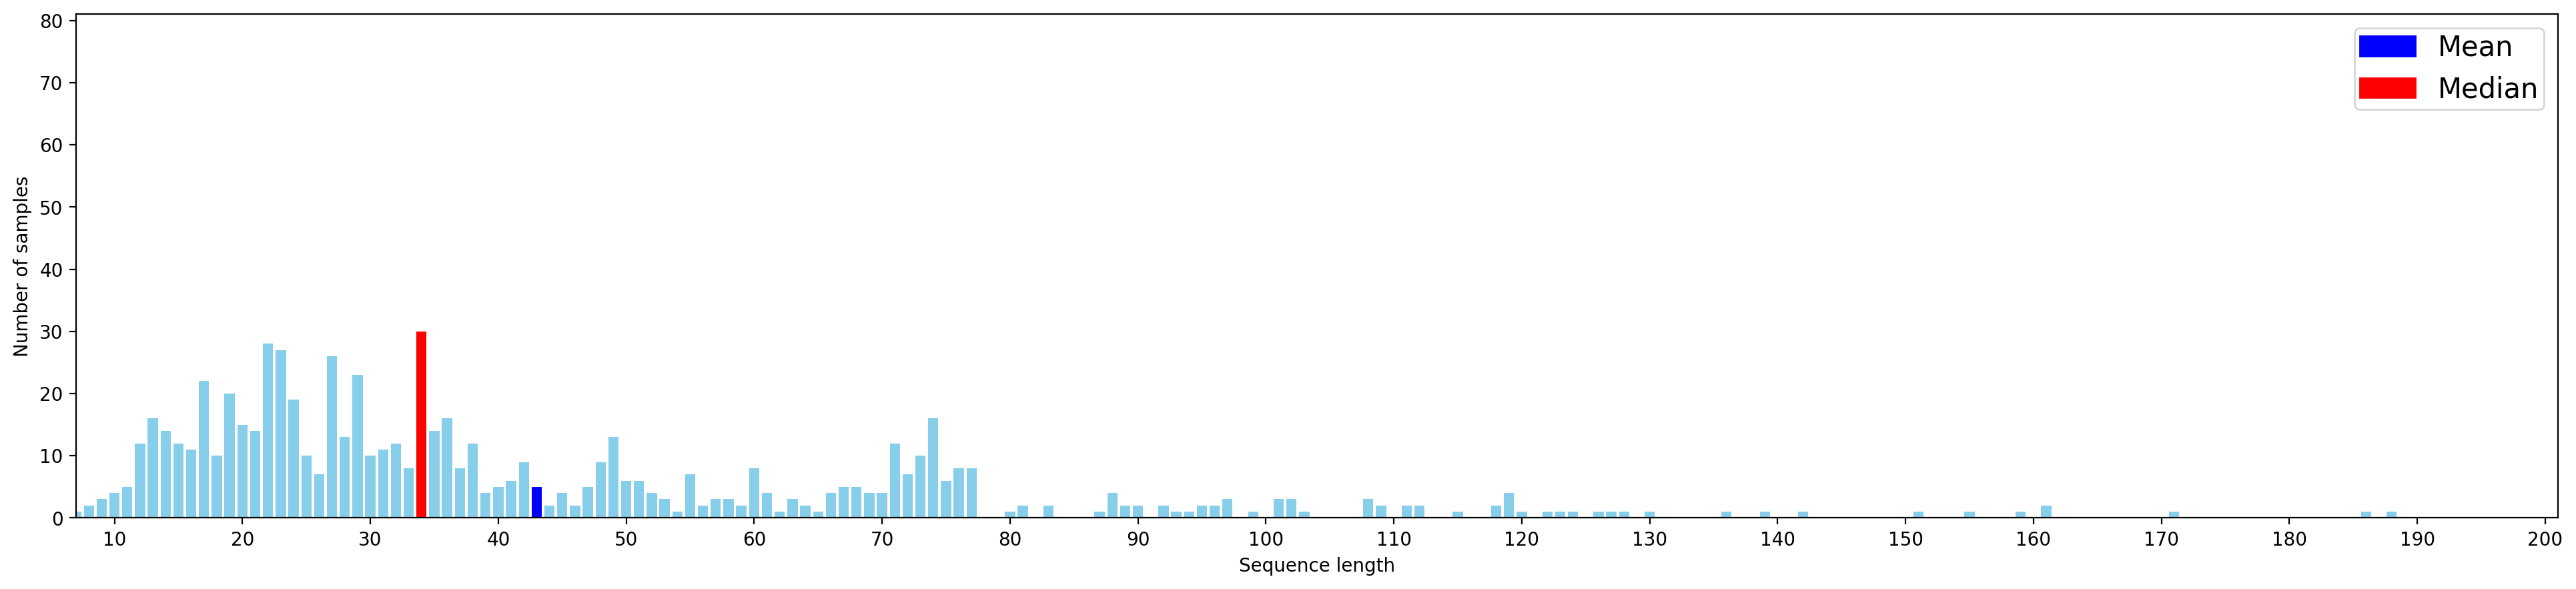
\includegraphics[width=\linewidth]{pics/plot_mps_distr.png}}
\caption{Analysis of Genegram-mps model compared with other tools }
\label{plots_pks}
\end{figure} 

As for functional tests, we similarly measured the prediction quality for three types of base pairs (table~\ref{table_mps}). Contacts belonging to multiplets are usually unstable, therefore, the ability of Genegram-mps model to predict multiplets resulted in high prediction accuracy for uncanonical base pairs. The definition of pseudoknot in the context of the multipletted structures is quite confusing, so, the estimation of pseudoknots was not run in this case. Instead of this, we provide the results of multiplets prediction. Note that there can be different ways of multiplets estimation and we choose two options for analysis: multiplets contacts (the amount of correct predictions among all contacts belonging to all multiplets in dataset) and multiplets pairs (the amount of correctly detected pairs $(i_1, j_1)$, $(i_2, j_2)$, where $i_1 = i_2$ or $i_1 = j_2$ or $j_1 = i_2$ or $j_1 = j_2$). The results of these tests are presented in the same table~\ref{table_mps}. It can be seen that all tools except Genegram are able to predict at most one contact of the multiplet pair and Genegram-mps model not only shows the highest contacts prediction score but also detects several paired interactions. However, the numbers are questionable so far, thus we introduce this model as a discussion about the possibilities of our approach rather than a final result.

\begin{table}[h!]
\centering
\caption{Genegram-mps and other models quality criteria measured on valid set}
\ra{1.4}
\begin{tabular}{@{}lccccccc@{}}\toprule
& \multicolumn{2}{c}{Multiplets} & \phantom{abc}& \multicolumn{3}{c}{Base pairs} \\
& Contacts & Pairs  && Watson-Crick & GU & Others \\ \cmidrule{2-3} \cmidrule{5-7} 
Genegram-mps  & 125 & 15 && 666 & 64 & 77 \\
SPOT-RNA & 101 & 0 && 680 & 64 & 44 \\
Ipknot & 67 & 0 && 630 & 56 & 0 \\
Knotty & 79 & 0 && 651 & 61 & 0 \\
RNAstructure & 73 & 0 && 643 & 62 & 0 \\
PknotsRG & 70 & 0 && 653 & 55 & 0 \\
HotKnots & 75 & 0 && 656 & 58 & 0 \\
\bottomrule
Expected & 448 & 395 && 863 & 132 & 316 \\
\bottomrule
\end{tabular}
\label{table_mps}
\end{table}

\subsubsection{Global tests}
In the previous sections we estimated three Genegram models separately on their validation sets and in this section, we provide some global tests for all the tools.

Due to the similar composition of training and validation sets for each model, the high results on validation make no reference to the general model quality, therefore, we downloaded several comparative and laboratory RNA secondary structure databases and evaluated Genegram models along with other tools on such data. These databases do not contain only purely selected structures, moreover, huge comparative databases usually aggregate a lot of homologous sequences with repetitive structural patterns, however, this experiment should check all models behavior on row data from various sources as opposed to the careful estimation on clean structures presented in the previous sections. We selected the following databases: CRW~\cite{cannone2002comparative}, Sprinzl~\cite{sprinzl1998compilation}, SRP~\cite{zwieb1992signal}, Rfam~\cite{griffiths2003rfam}, PDB~\cite{berman2000protein} (only single-chain samples without unmodelled bases) and Pseudobase~\cite{van2000pseudobase}. Note that most of these samples are completely new, however, some sequences or even databases could be previously used for some models training (e.g. Pseudobase was included in Genegram-pks training set). Table~\ref{table_all} represents the estimation of three Genegram models along with other tools by mean $F1$ score on all databases and the last column shows the mean $F1$ value among total samples. It can be seen that in most cases our models show adequate numbers regarding other tools, so, we can state that all neural networks generalize well on new datasets.

\begin{table}
\centering
\caption{All models estimation by $F1$ metrics on different databases}
\ra{1.4}
\begin{tabular}{@{}lcccccccc@{}}\toprule
& CRW & Sprinzl & SRP & Rfam & PDB & Pseudobase  & All data \\ \cmidrule{2-8} 
Genegram-main  & 69 & 73 & 59 & 43 & 74 & 42 & 69 \\
Genegram-pks  & 66 & 72 & 56 & 48 & 74 & 81 & 68 \\
Genegram-mps  &  &  &  &  &  &  &  \\
SPOT-RNA & 89 & 88 & 65 & 72 & 81 & 70 & 87 \\
Ipknot & 74 & 79 & 49 & 64 & 76 & 59 & 75 \\
Knotty & 74 & 75 & 63 & 63 & 79 & 76 & 74 \\
RNAstructure & 66 & 69 & 56 & 64 & 77 & 62 & 67 \\
PknotsRG & 62 & 61 & 65 & 66 & 79 & 77 & 62 \\
HotKnots & 61 & 60 & 66 & 66 & 78 & 61 & 61 \\
\bottomrule
Total samples & 11606 & 8777 & 360 & 1043 & 290 & 357 & 22433 \\
\bottomrule
\end{tabular}
\label{table_all}
\end{table}

Finally, we measured the time required for each tool to process fasta file with 100 RNA sequences and return secondary structure prediction for each sequence in its default output format. These tests were carried out on the workstation with the following characteristics: Ubuntu 20.04.2 LTS, Intel Core i5-10210U CPU 1.60GHz, NVIDIA GeForce MX250 GPU, and 7.5 GB RAM. We prepared two datasets by randomly selecting sequences from RNA STRAND database: the first set contained 100 sequences having lengths up to 100 and the second one --- 100 sequences with lengths up to 200. Table~\ref{table_time} shows the results of a performance experiment for such two fasta files. Genegram and SPOT-RNA were launched on GPU and the other tools have only CPU versions. It can be seen that the elapsed time spread among tools is quite big, moreover, several tools significantly lose in performance while processing longer sequences since various secondary structure prediction techniques may have completely different algorithmic complexity. However, Genegram shows an adequate performance due to the effective use of GPGPU in the parsing algorithm as well as in the neural network.

\begin{table}
\centering
\caption{Tools time performance on 100 sequences}
\ra{1.4}
\begin{tabular}{@{}lccc@{}}\toprule
& \multicolumn{2}{c}{\phantom{abc}  \phantom{abc}  \phantom{abc} Elapsed time, seconds}  \\
& Lengths 1-100 && Lengths 1-200  \\ \cmidrule{2-2} \cmidrule{4-4} 
Genegram & 28 && 39 \\
SPOT-RNA & 68 && 235 \\
Ipknot & 1 && 1 \\
Knotty & 283 && 3050 \\
RNAstructure & 10 && 15 \\
PknotsRG & 15 && 95 \\
HotKnots & 37 && 366 \\
\bottomrule
\end{tabular}
\label{table_time}
\end{table}

\section{Заключение}
\section{Conclusion}

In this paper we present a library for sparse Boolean linear algebra which implements such basic operations as matrix-matrix multiplication and element-wise matrix-matrix addition in both Cuda and OpenCL.
Evaluation shows that our Boolean-specific implementations faster and require less memory than generic, not the Boolean optimized, operations from state-of-the-art libraries. 
Thus, the specialization of operations for this data type makes sense. 

The first direction of the future work is to integrate all parts (OpenCL and Cuda backends) into a single library and improve its documentation and prepare to publish.
Moreover, it is necessary to extend the library with other operations, including matrix-vector operations, masking, and so on.
As a result a Python package should be published.

Another important step is to evaluate the library on different algorithms and devices.
Namely, algorithms for RPQ and CFPQ should be implemented and evaluated on related data sets.
Also, it is necessary to evaluate OpenCL version on FPGA which may require additional technical effort and code changes.

Finally, we plan to discuss with GraphBLAS community possible ways to use our library as a backend for GraphBLAST or SuiteSparse in case of Boolean computations.
Moreover, it may be possible to use implemented algorithms as a foundation for generalization to arbitrary semirings.


% \nocite{*}
\setmonofont[Mapping=tex-text]{CMU Typewriter Text}
\bibliographystyle{ugost2008ls}
\bibliography{vkr}
\end{document}
